\documentclass[11pt]{article}
\usepackage{spikey}
\usepackage{amsmath}
\usepackage{amssymb}
\usepackage{soul}
\usepackage{float}
\usepackage{graphicx}
\usepackage{hyperref}
\usepackage{xcolor}
\usepackage{chngcntr}
\usepackage{mathrsfs}
\usepackage{centernot}
\usepackage[shortlabels]{enumitem}

\usepackage[margin=1truein]{geometry}

\title{ECO374 Winter 2019 \\ Forecasting and Time Series Econometrics}
\date{\today}
\author{Tianyu Du}

\counterwithin{equation}{section}
\counterwithin{theorem}{section}
\counterwithin{lemma}{section}
\counterwithin{corollary}{section}
\counterwithin{proposition}{section}
\counterwithin{remark}{section}
\counterwithin{example}{section}
\counterwithin{figure}{section}

\usepackage[
    type={CC},
    modifier={by-nc},
    version={4.0},
]{doclicense}

\begin{document}
	\maketitle
	\doclicenseThis
	\begin{itemize}
		\item GitHub: \url{https://github.com/TianyuDu/Spikey_UofT_Notes}
		\item Website: \url{TianyuDu.com/notes}
	\end{itemize}
	\tableofcontents
	\newpage
	
	\section{Introduction and Statistics Review}
		\subsection{Definitions}
		\begin{definition}
			Given random variable $X$, the $k^{th}$ \textbf{non-central moment} is defined as
			\begin{equation}
				\expect{X^k}
			\end{equation}
		\end{definition}
		
		\begin{definition}
			Given random variable $X$, the $k^{th}$ \textbf{central moment} is defined as
			\begin{equation}
				\expect{(X - \expect{X})^k}
			\end{equation}
		\end{definition}
		
		\begin{remark}
			Moments of order higher than a certain $k$ may not exist for certain distribution.
		\end{remark}
		
		\begin{definition}
			Given the \textbf{joint density} $f(X,Y)$ of two \emph{continuous} random variables, the \textbf{conditional density} of random $Y$ conditioned on $X$ is 
			\begin{equation}
				f_{Y|X}(y|x) = \frac{f_{Y,X}(y, x)}{f_X(x)}
			\end{equation}
		\end{definition}
		
		\begin{definition}
			Given \emph{discrete} random variables $X$ and $Y$, the \textbf{conditional density} of $Y$ conditioned on $X$ is defined as 
			\begin{equation}
				P(Y=y|X=x) = \frac{P(Y=y \land X=x)}{P(X=x)}
			\end{equation}
		\end{definition}
		
		\subsection{Multiple Linear Regression}
		\begin{assumption} Assumptions on linear regression on time series data:
			\begin{enumerate}[(i)]
				\item \textbf{Linearity}
					\begin{equation}
						Y = \beta_0 + \beta_1 X_1 + \dots + \beta_k X_k + u
					\end{equation}
				\item \textbf{Zero Conditional Mean}
					\begin{equation}
						\expect{u|X_1, X_2, \dots, X_k} = 0
					\end{equation}
				\item \textbf{Homoscedasitcity}
					\begin{equation}
						\var{u|X_1, X_2, \dots, X_k} = \sigma^2_u
					\end{equation}
				\item \textbf{No Serial Correlation}
					\begin{equation}
						Cov(u_t, u_s) = 0\ \forall t \neq s \in \Z
					\end{equation}
				\item \textbf{No Perfect Collinearity}
				\item \textbf{Sample Variation in Regressors}
					\begin{equation}
						\var{X_j} > 0\ \forall j
					\end{equation}
			\end{enumerate}
		\end{assumption}
		
		\begin{theorem}[Gauss-Markov Theorem]
			Under assumptions 1.1, the OLS estimators $\hat{\beta}_j$ are \emph{best linear unbiased estimators} of the unknown population regression coefficients $\beta_j$.
		\end{theorem}
		
		\begin{remark}
			\hl{The \emph{no serial correlation} assumption is typically not satisfied for time series data.} And the \emph{linearity} assumption is also too restrictive for time series featuring complex dynamics. Hence, for time series data we typically use other models than linear regression with OLS.
		\end{remark}
		
	\section{Statistics and Time Series}
		\subsection{Stochastic Processes}
		\begin{definition}
			A \textbf{stochastic process} (or \textbf{time series process}) is a family (collection) random variables indexed by $t \in \mc{T}$ and defined on some given probability space $(\Omega, \mc{F}, P)$.
			\begin{equation}
				\{Y_t\}_{t \in \mc{T}} = Y_1, \dots, Y_T
			\end{equation}
		\end{definition}
		
		\begin{definition}
			The function from $\mc{T}$ to $\R$ which assigns to each point in time $t \in \mc{T}$ the realization of the random variable $Y_t$, $y_t$ is called a \textbf{realization}\footnote{It's also called a \textbf{trajectory} or an \textbf{outcome}} of the stochastic process.
			\begin{equation}
				\{y_t\} = y_1, \dots, y_T
			\end{equation}
			Such realization is called is a \textbf{time series}.
		\end{definition}
		
		\begin{definition}
			A \textbf{time series model} or a \textbf{model} for the observations, $\{y_t\}$, is a specification of the \emph{joint distribution} of $\{Y_t\}$ for which $\{y_t\}$ is a realization.
		\end{definition}
		
		\begin{assumption}
			The \textbf{ergodicity} assumption requires the observations cover in principle all possible events.
		\end{assumption}
		
		\begin{definition}
			A stochastic process $\{Y_t\}$ is \textbf{first order strongly stationary} if all random variables $Y_t \in \{Y_t\}$ has the \emph{exactly same probability density function}.
		\end{definition}
		
%		\begin{definition}[1.7]
%			A stochastic process $\{Y_t\}$ is \textbf{strictly stationary} if for all $h, n \geq 1$, $(Y_1,\dots,Y_n)$ and $(Y_{1+h}, \dots, Y_{n+h})$ have the same distribution.
%		\end{definition}
		
		\begin{definition}
			A stochastic process $\{Y_t\}$ is \textbf{first order weakly stationary} if
			\begin{equation}
				\forall t \in \mc{T},\ \mu_{Y_t} \equiv \expect{Y_t} = \bar{\mu}
			\end{equation}
		\end{definition}
		
		\begin{definition}
			A stochastic process $\{Y_t\}$ is \textbf{second order weakly stationary}, or \hl{\textbf{covariance stationary}} if all random variables $\{Y_t\}$ have the same mean and variance. And the covariances do not depend on $t$.
			That's, for all $t \in \mc{T}$,
			\begin{enumerate}[(i)]
				\item $\expect{Y_t} = \mu\ \forall t$ constant;
				\item $\var{Y_t} = \sigma^2 < \infty\ \forall t$ constant;
				\item $Cov(Y_t, Y_s) = Cov(Y_{t+r}, Y_{s+r})\ \forall t,s,r\in \Z$
			\end{enumerate}
		\end{definition}
		
		\subsection{Auto-correlations}
		
		\begin{definition}
			Let $\{Y_t\}$ be a stochastic process with $\var{Y_t} < \infty\ \forall t \in \mc{T}$, the \textbf{auto-covariance function} is defined as
			\begin{gather}
				\gamma_Y(t, s) := Cov(Y_t, Y_s) \\
				= \expect{(Y_t - \expect{Y_t})(Y_s - \expect{Y_s})} \\
				= \expect{Y_t Y_s} - \expect{Y_t} \expect{Y_s}
			\end{gather}
		\end{definition}
		
		\begin{lemma}
			If $\{Y_t\}$ is stationary, then the auto-covariance function only depends on \emph{the lag between two inputs}, and does not depend on specific time point $t$. We can write the $h \in \Z$ degree auto-covariance as 
			\begin{equation}
				\gamma_Y(h) := \gamma_X(t, t+h)\ \forall t \in \mc{T}
			\end{equation}
		\end{lemma}
	
		\begin{proposition}
			By the symmetry of covariance, 
			\begin{equation}
				\gamma_Y(h) = \gamma_Y(-h)
			\end{equation}
		\end{proposition}
		
		\begin{definition}
			The \textbf{auto-correlation coefficient} of order $k$ is given by
			\begin{equation}
				\rho_{Y_t, Y_{t-k}} = \frac{Cov(Y_t, Y_{t-k})}{\sqrt{\var{Y_t}}\sqrt{\var{Y_{t-k}}}}
			\end{equation}
		\end{definition}
		
		\begin{definition}
			Let $\{Y_t\}$ be a \emph{covariance stationary process} and the \textbf{auto-correlation function} (ACF) is a mapping from \emph{order} of auto-correlation coefficient to the coefficient $\rho_Y: k \to \rho_{Y_t, Y_{t-k}}$, defined as
			\begin{equation}
				\rho_Y(k) \equiv \frac{\gamma(k)}{\gamma(0)} = corr(Y_{t + k}, Y_t)
			\end{equation}
			notice the choice of $t$ does not matter, by definition of covariance stationary process.
		\end{definition}
		
		\begin{proposition}
			Note that 
			\begin{equation}
				\rho_k = \rho_{-k} = \rho_{|k|}
			\end{equation}
			so the ACF for stationary process can be simplified to a mapping 
			\begin{equation}
				\rho: k \to \rho_{|k|}
			\end{equation}
		\end{proposition}
		
		\begin{remark}
			\hl{Strong stationarity is difficult to test so we will focus on weak(covariance) stationarity only.}
		\end{remark}
		
		\begin{proposition}
			For a non-stationary stochastic process $\{Y_t\}$,
			\begin{itemize}
				\item $\{\Delta Y_t\}$ becomes \emph{first order weakly stationary};
				\item and $\{\Delta \log(Y_t)\}$ becomes \emph{second order weakly stationary (covariance stationary)}.
			\end{itemize}
			\begin{figure}[h]
				\centering
				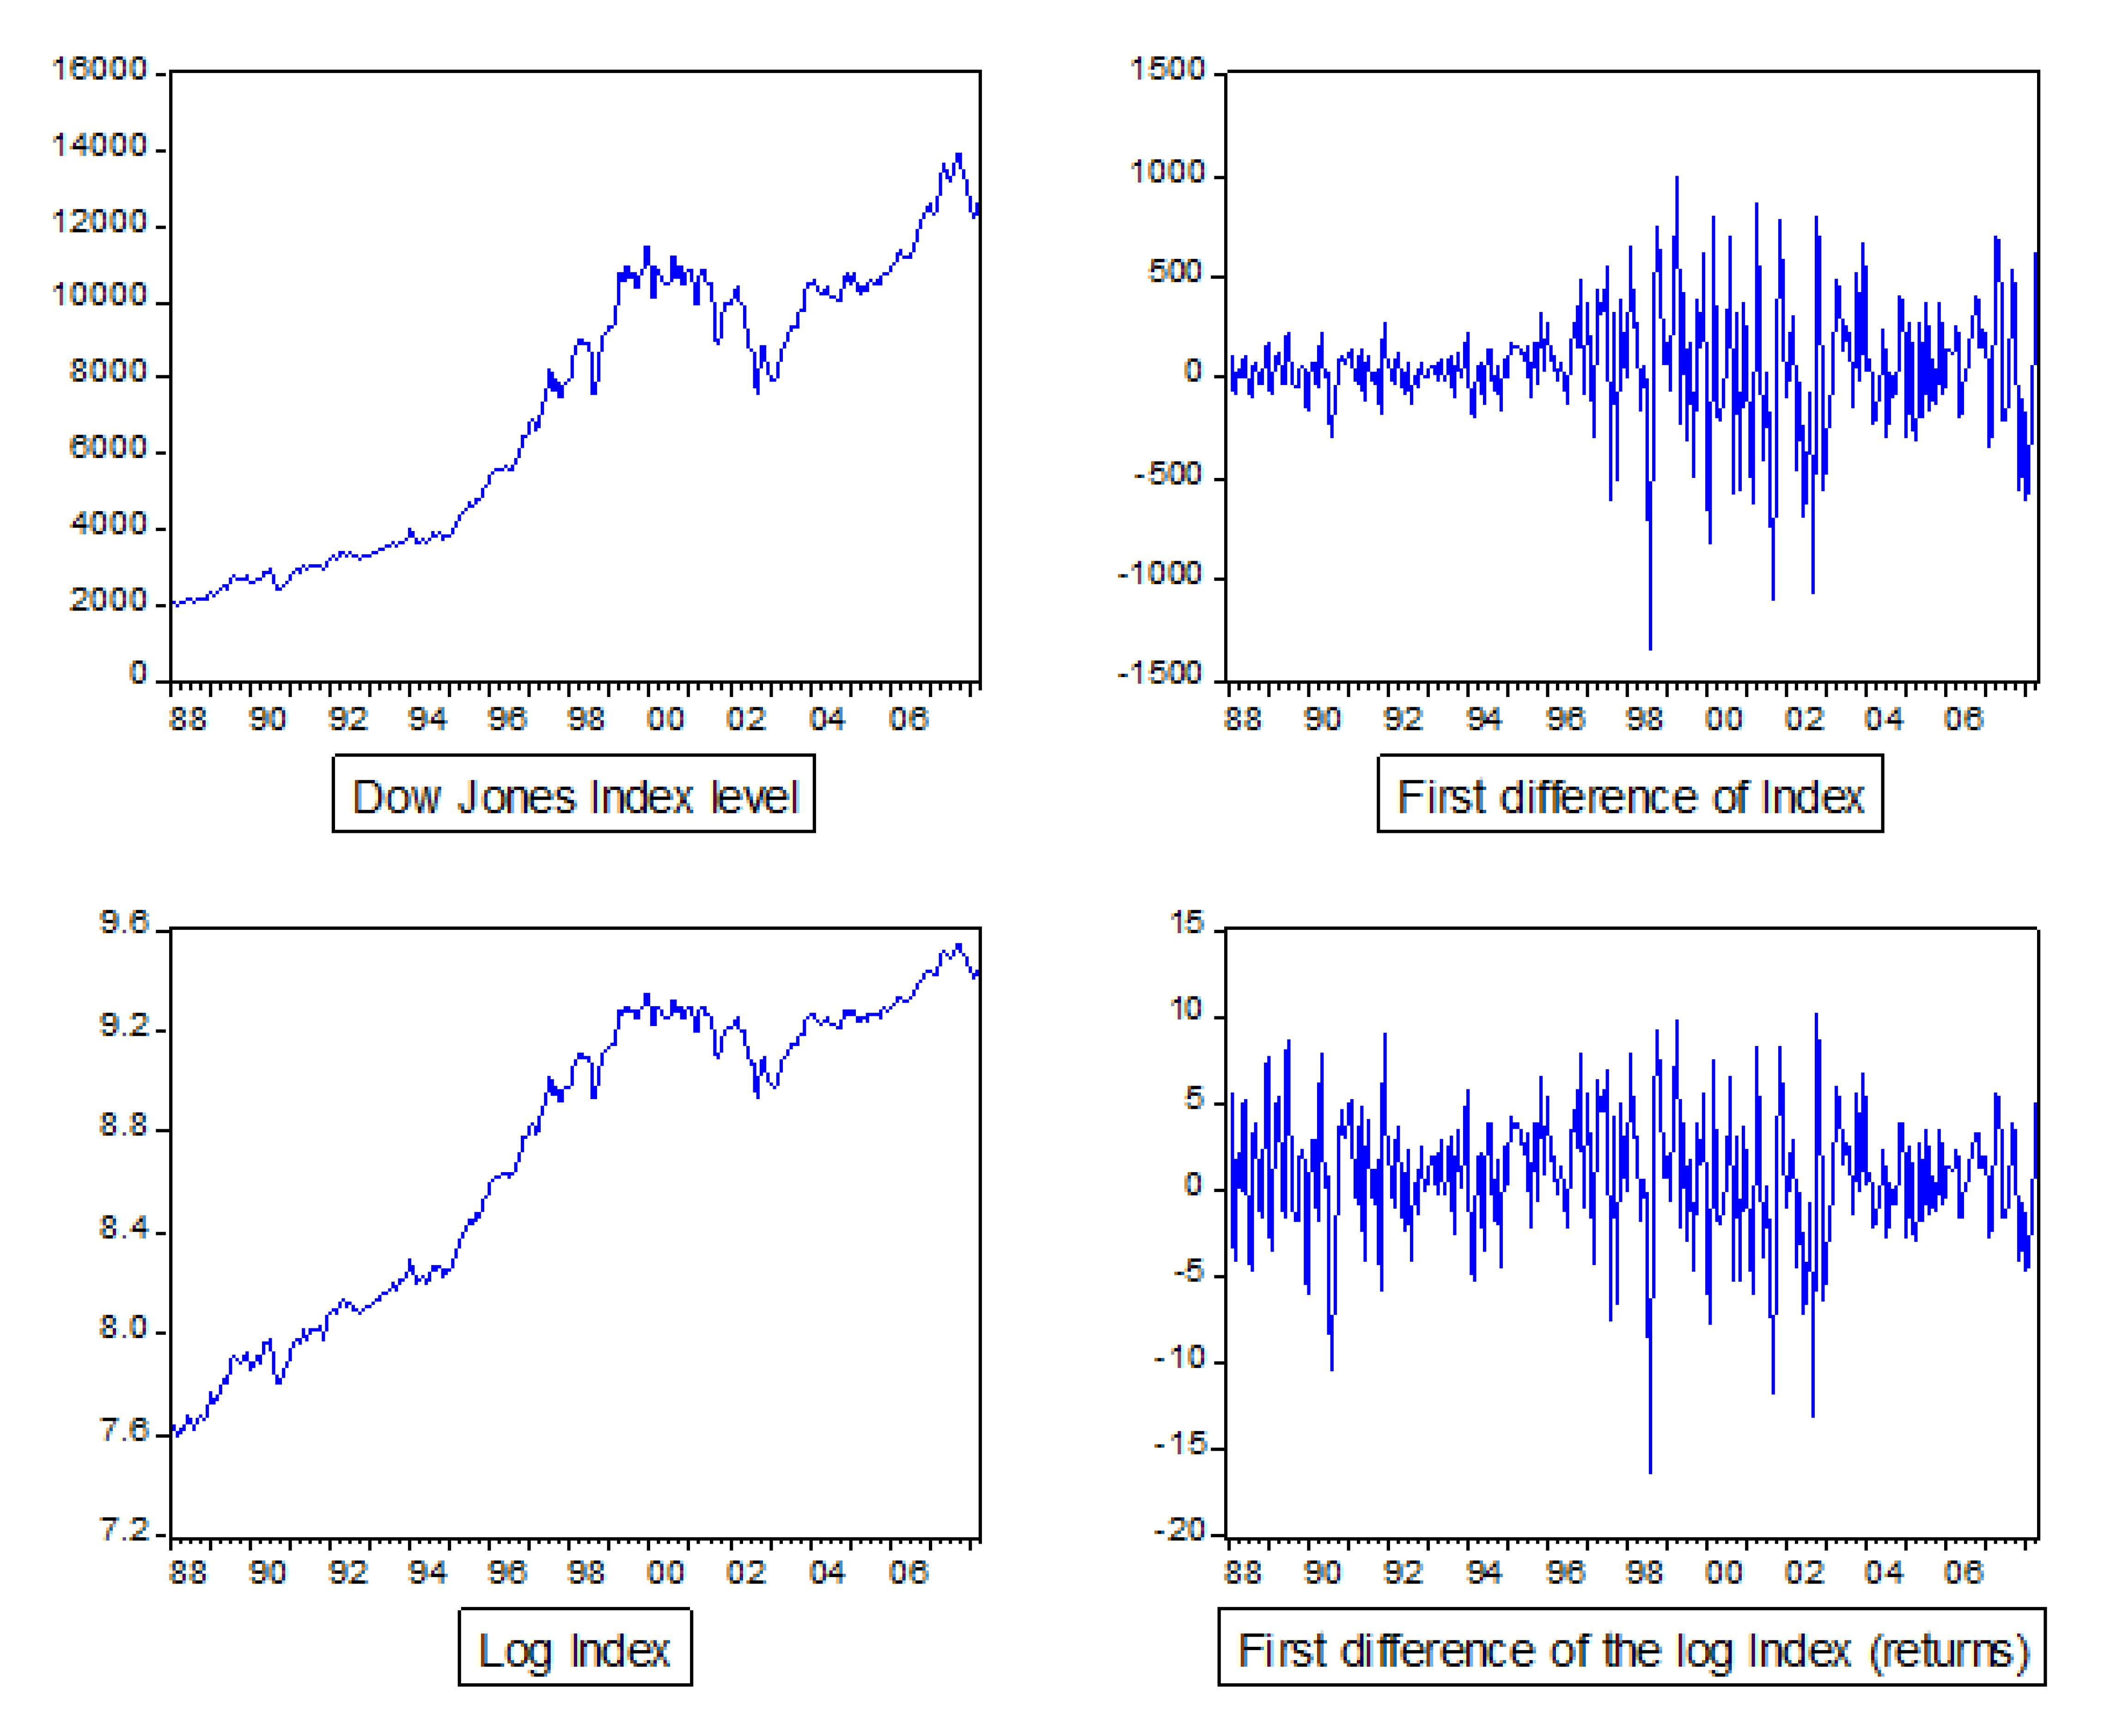
\includegraphics{figures/2_1}
			\end{figure}
		\end{proposition}
		
		\begin{definition}[1.8]
			A stochastic process $\{Y_t\}$ is called a \textbf{Gaussian process} if the distribution for all \emph{finite} dimensional segments from the process are \ul{multivariate normal}. That's
			\begin{gather}
				\forall n \in \Z_{++},\ \forall (t_1, \dots, t_n) \in \mc{T}^n, (Y_{t_1}, \dots, Y_{t_n}) \sim \mc{N}(\bs{\mu}, \Sigma)
			\end{gather}
		\end{definition}
		
		\begin{notation}
			Consider the problem of forecasting $Y_{T+1}$ from observations $\{Y_t\}_{t=1}^{T}$, the \emph{best linear predictor} is denoted as
			\begin{equation}
				\mathbb{P}_T Y_{T+1} = \sum_{i=1}^{T} a_i L^i Y_{T+1}
			\end{equation}
			And $Y_{T+1}$ can be expressed as
			\begin{equation}
				Y_{T+1} = \mathbb{P}_T Y_{T+1} + \varepsilon_{T+1}
			\end{equation}
			where $\varepsilon_{T+1}$ denotes the forecast error which is assumed to be \emph{uncorrelated} with $Y_T, \dots, Y_1$.
		\end{notation}
		
		\begin{definition}[3.3]
			The \textbf{partial auto-correlation function} (PACF) $r(h)$ with $h \in \Z_{\geq 0}$ of a \emph{stationary} process is defined as 
			\begin{gather}
				r(0) = 1 \\
				r(1) = corr(Y_2, Y_1) = \rho(1) \\
				r(h) = corr\Big(Y_{h+1} - \mathbb{P}(Y_{h+1}|1,Y_2, \dots, Y_h), X_1 - \mathbb{P}(Y_1|1,Y_2,\dots,Y_h)\Big)
			\end{gather}
		\end{definition}
		
		\begin{remark}[Interpretation of PACF]
		Partial auto-correlation $r(k)$ only measures correlation between two variables $Y_t$ and $Y_{t+k}$ while \emph{controlling intermediate variables} $(Y_{t+1}, \dots, Y_{t+k-1})$.
		\end{remark}
		
		\begin{remark}
			\hl{Partial auto-correlation can be interpreted as the estimated coefficients when regressing $Y_t$ on its lagged values.}
		\end{remark}
		
		\begin{remark}AR and MA signatures on ACF and PACF plot.\footnote{Zero here means statistically insignificant.}
			\begin{table}[h]
				\centering
				\begin{tabular}{l|c|c}
					processes & ACF ($\rho$) & PACF ($r$) \\
					\hline
						AR($p$) & 
						\begin{tabular}{@{}c@{}}Declines exponentially \\(monotonic or oscillating) to zero\end{tabular} & 
						$r(h) = 0\ \forall h > p$\\
					\hline
						MA($q$) &
						$\rho(h) = 0\ \forall h > q$ &
						\begin{tabular}{@{}c@{}}Declines exponentially \\(monotonic or oscillating) to zero\end{tabular}
				\end{tabular}
			\end{table}
		\end{remark}
	
	\subsection{Test for Auto-correlation}
		\par To test single auto-correlation with 
		\begin{equation}
			H_0: \rho_k = 0
		\end{equation}
		we can use usual t-statistic.\\
		While testing the \hl{joint hypothesis}
		\begin{equation}
			H_0: \rho_1 = \rho_2 = \dots = \rho_k = 0
		\end{equation}
		we are using the \textbf{Ljung-Box Q-statistic}:
		\begin{equation}
			Q_k = T(T+1) \sum_{j=1}^k \frac{\hat{\rho}_j^2}{T-j} \sim \chi_k^2
		\end{equation}
	\subsection{Causality and Invertibility (Optional)}
	\subsubsection{Causality}
		\begin{definition}[Causality]
			An ARMA($p, q$) process $\{Y_t\}$ with 
			\begin{equation}
				\Phi(L)Y_t = \Theta(L)\varepsilon_t
			\end{equation}
			is called \textbf{causal with respect to} $\{\varepsilon_t\}$ if there exists a sequence $\Psi \equiv \{\psi_j\}$ with the property $\sum_{j=0}^\infty |\psi_j| < \infty$ such that 
			\begin{equation}
				Y_t = \Psi(L) \varepsilon_t\ \tx{ with } \psi_0 = 1
			\end{equation}
			where $\Psi(L) \equiv \sum_{j=0}^\infty \psi_j L^j$. The above equation is referred to as the \textbf{causal representation} of $\{Y_t\}$ with respect to $\{\varepsilon_t\}$.
		\end{definition}
		
		\begin{proposition}
			\hl{By the definition of causality, a pure MA process (which is stationary) is naturally a causal representation with respect to it's own error term $\{\varepsilon_t\}$.}
		\end{proposition}
		
		\begin{theorem}
			Let $\{Y_t\}$ be an ARMA($p, q$) process with 
			\begin{equation}
				\Phi(L)Y_t = \Theta(L)\varepsilon_t
			\end{equation}
			such that polynomials $\Phi(z)$ and $\Theta(z)$ have no common roots.\\
			Then $\{Y_t\}$ is causal with respect to $\{\varepsilon_t\}$ \ul{if and only if} \hl{all roots of $\red{\Phi(z)}$ are \textbf{outside} the unit circle}. The coefficients $\Psi$ are then uniquely defined by identity
			\begin{equation}
				\Psi(z) = \sum_{j=0}^\infty \psi_j z^j = \frac{\Theta(z)}{\Phi(z)}
			\end{equation}
		\end{theorem}
	\subsubsection{Invertibility}
	\begin{definition}[Invertibility]
		An ARMA($p, q$) process for $\{Y_t\}$ satisfying
		\begin{equation}
			\Phi(L)Y_t = \Theta(L)\varepsilon_t
		\end{equation}
		is called \textbf{invertible} with respect to $\{\varepsilon\}$ if and only if there exists a sequence $\Pi$ with the property $\sum_{j=0}^\infty |\pi_j| < \infty$ such that
		\begin{equation}
			\varepsilon_t = \sum_{j=0}^\infty \pi_j L^j Y_t
		\end{equation}
	\end{definition}
	
	\begin{proposition}
		\hl{By the definition of invertibility, a stationary auto-regressive process is naturally invertible with respect to it's own error term $\{\varepsilon_t\}$.}
	\end{proposition}
	
	\begin{theorem}
		Let $\{Y_t\}$ be an ARMA($p, q$) process with 
		\begin{equation}
			\Phi(L)Y_t = \Theta(L)\varepsilon_t
		\end{equation}
		Then $\{Y_t\}$ is invertible with  respect to $\{\varepsilon_t\}$ \ul{if and only if} \hl{all roots of $\red{\Theta(z)}$ are \textbf{outside} the unit circle}. And the coefficients of $\Pi \equiv \{\pi_j\}$ are then uniquely determined by the relation
		\begin{equation}
			\Pi(z) = \sum_{j=0}^\infty \pi_j z^j = \frac{\Phi(z)}{\Theta(z)}
		\end{equation}
	\end{theorem}
	
	\section{Forecasting Tools}
	\subsection{Information Set}
		\begin{definition}
			For stochastic process $\{Y_t\}$, the \textbf{information set} $I_t$ is the \emph{known time series} up to time $t$. It takes the form of a $n$-tuple $(y_{t_1}, y_{t_2}, \dots, y_{t_n})$ such that $t_n \leq t$ so the information set is \emph{certain} at time $t$.
		\end{definition}
		
		\begin{definition}
			A \textbf{forecast} $f_{t, h}$ is the image of a \emph{time series model} $g$ under given information set $I_t$. Specifically,
			\begin{equation}
				f_{t, h} = g(I_t) \in \R
			\end{equation}
		\end{definition}
	\subsection{Forecast Horizon}
		\begin{remark}
			\emph{Covariance stationary} processes are \textbf{short-memory processes}. More recent observation contains information far more relevant for the future than older information. \hl{Therefore, as a result, the forecast $f_{t, h}$ converges when $h \to \infty$.}
		\end{remark}
		
		\begin{remark}
			\emph{Non-stationary} processes are \textbf{long-memory processes} and older information is as relevant for the forecast as more recent information.
		\end{remark}
		\subsubsection{Forecasting Environments: \emph{Recursive}}
			\begin{enumerate}[(i)]
				\item \emph{Re-train} and predict with \emph{updated} information set;
				\item Advantageous if model is \emph{stable over time};
				\item Not robust to \hl{\emph{structural break}}. 
			\end{enumerate}
			\begin{figure}[H]
				\centering
				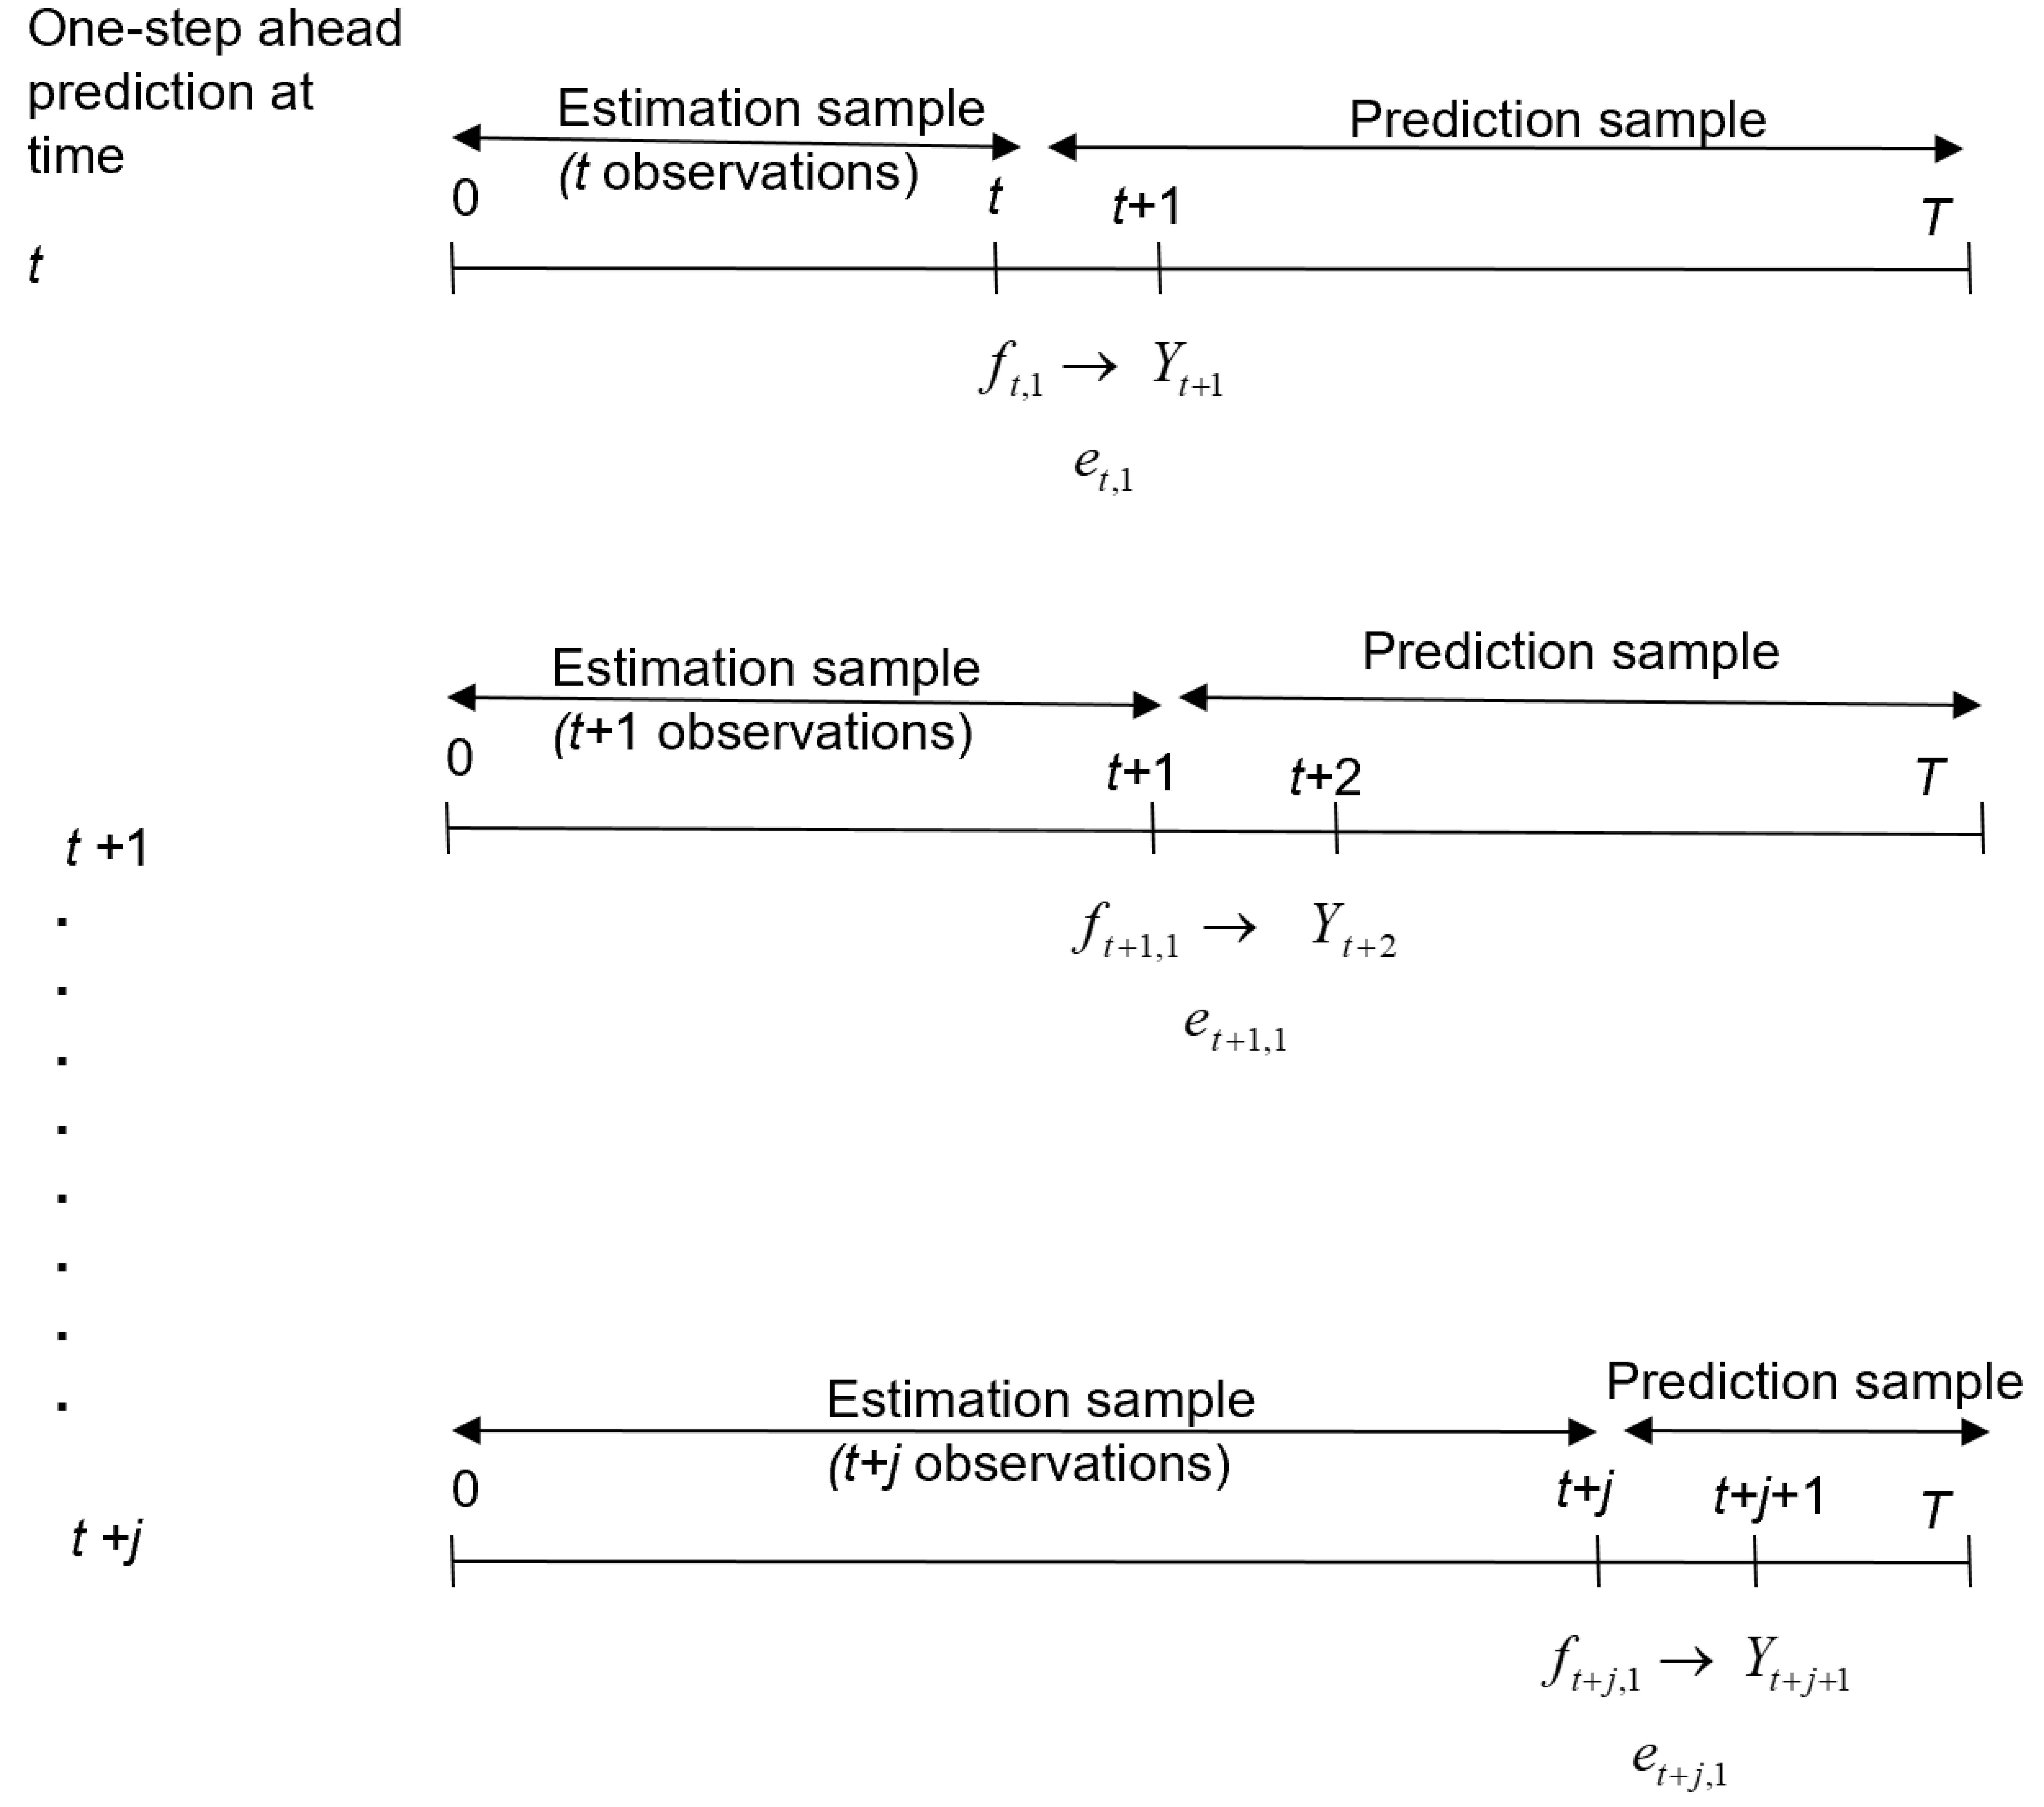
\includegraphics[width=0.5\linewidth]{figures/recursive_forecast}
				\caption{Recursive Forecasting Scheme}
			\end{figure}
		\subsubsection{Forecasting Environments: \emph{Rolling}}
			\begin{enumerate}[(i)]
				\item \emph{Re-train} and predict with \emph{updated but fixed-size} information set;
				\item Robust against \hl{\emph{structural breaks}};
				\item Not fully exploit information available.
			\end{enumerate}
			\begin{figure}[H]
				\centering
				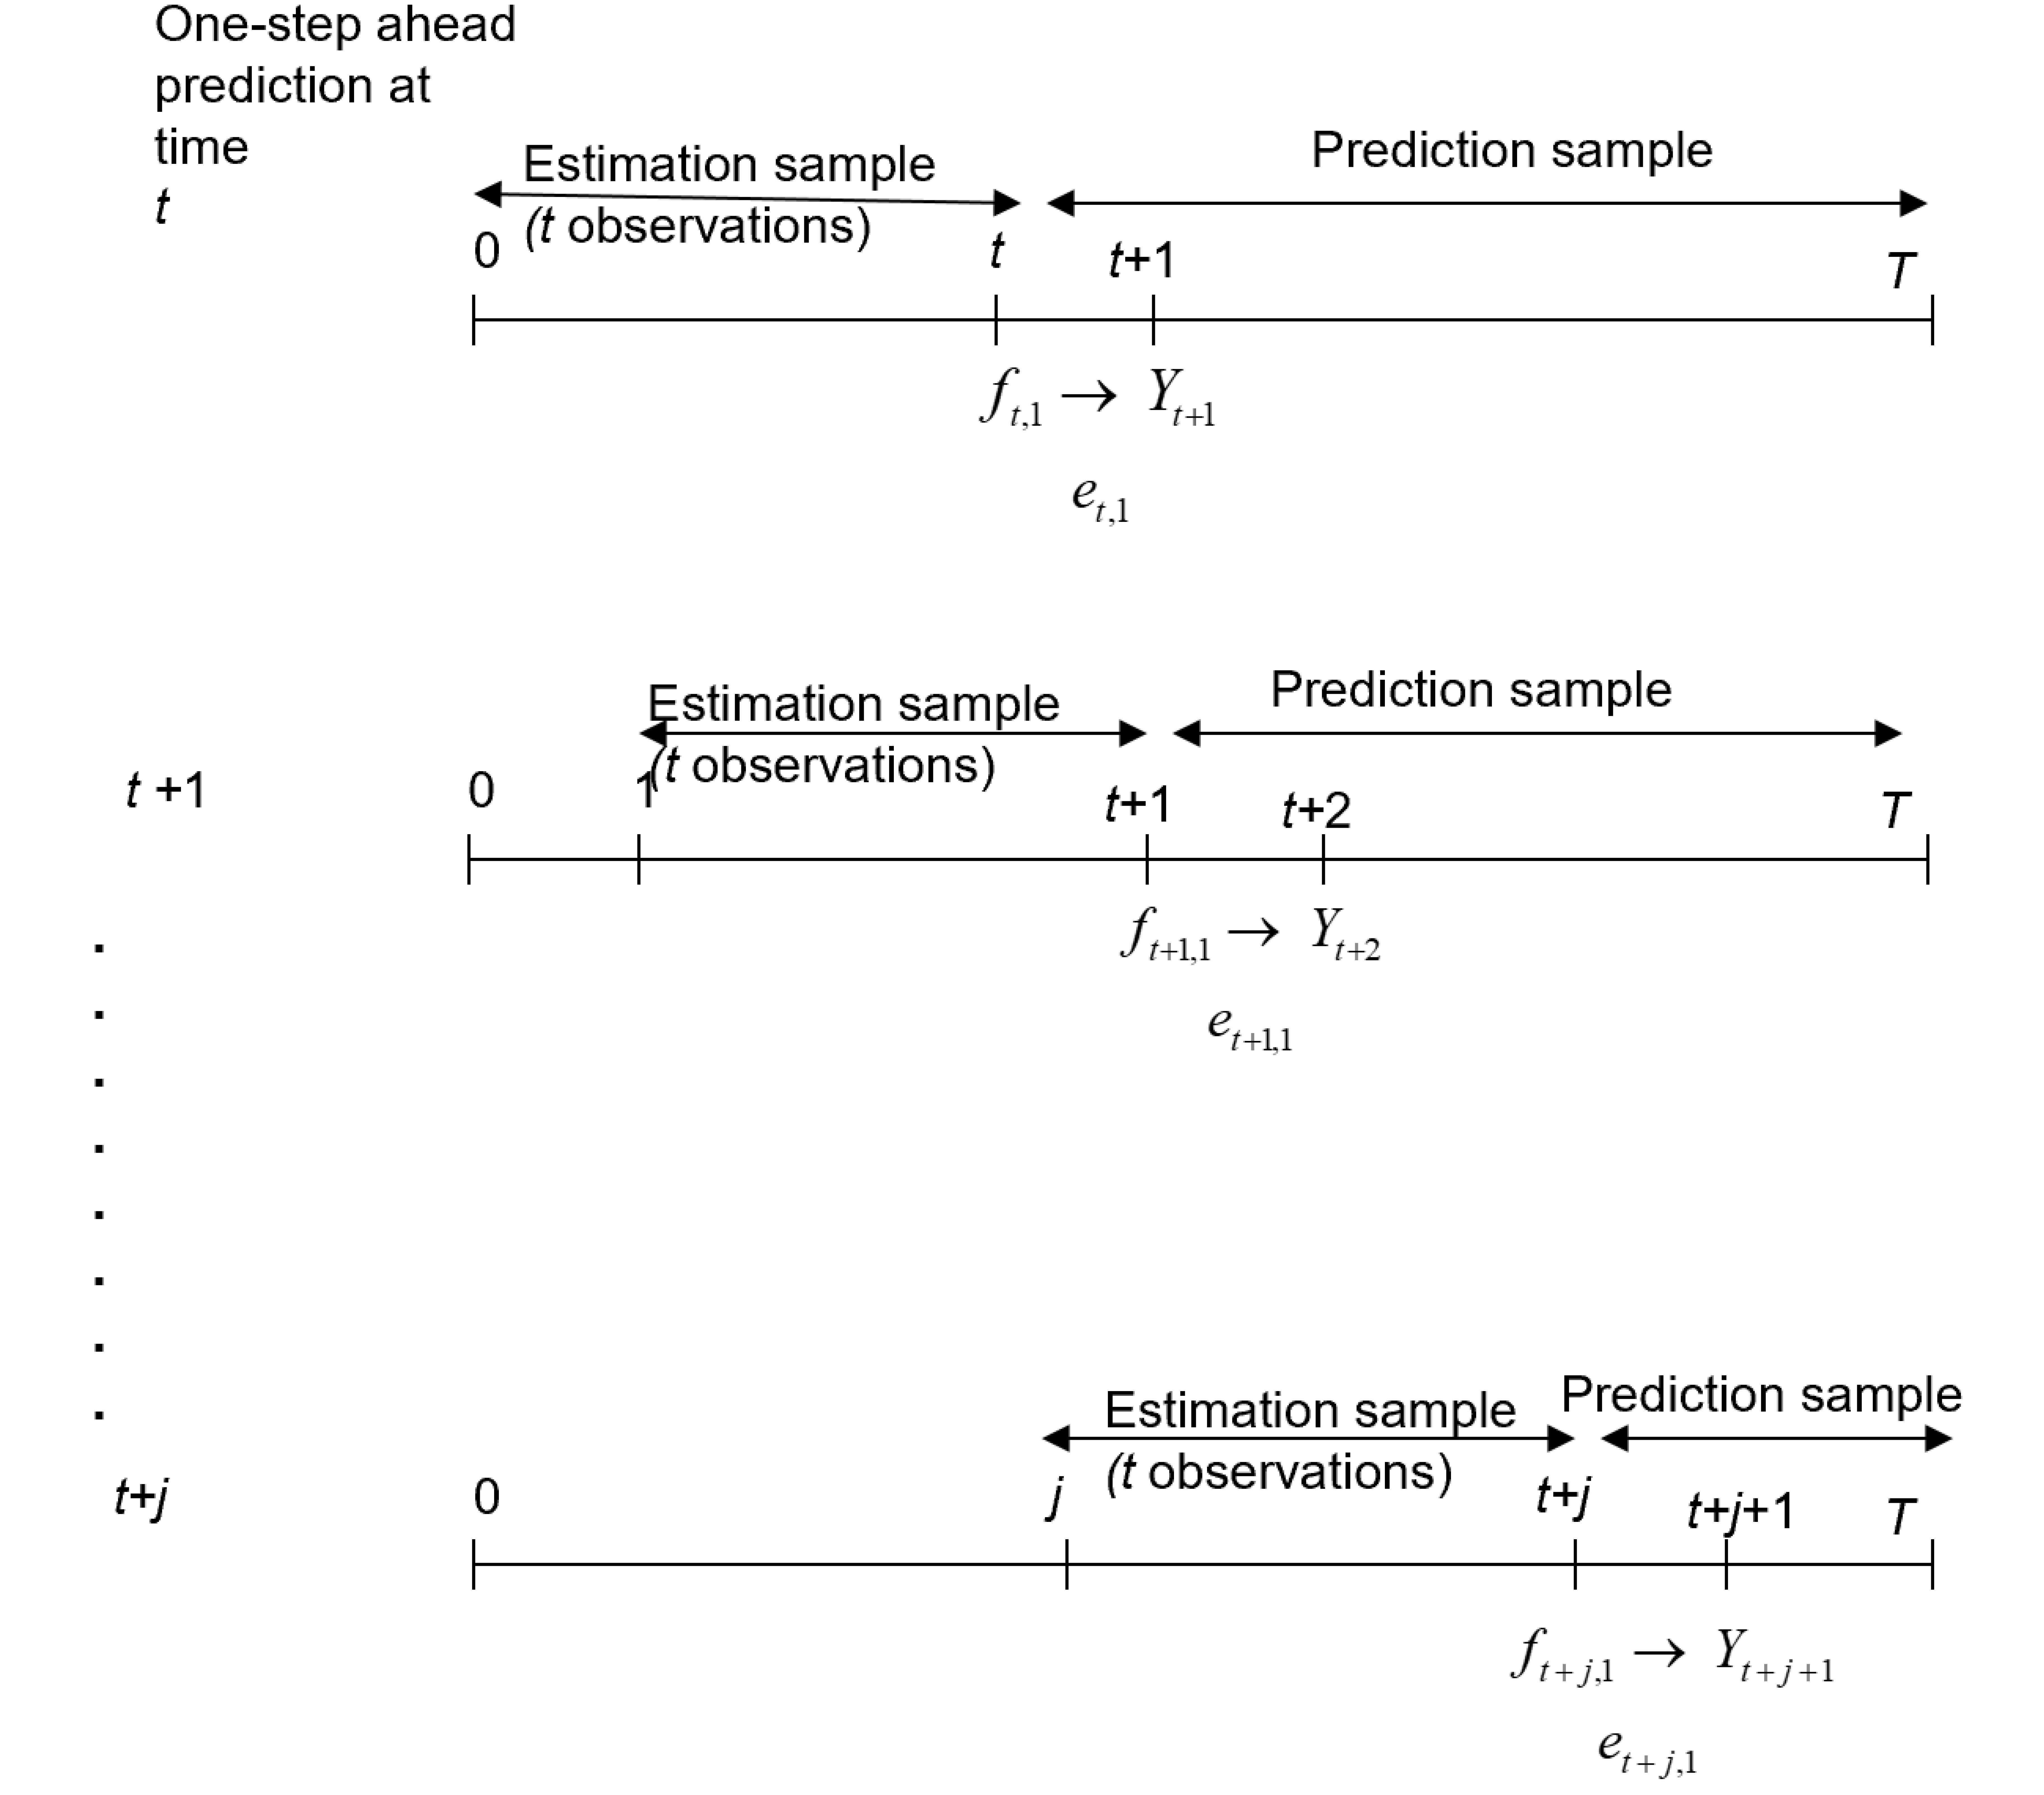
\includegraphics[width=0.5\linewidth]{figures/rolling_forecast}
				\caption{Rolling Forecasting Scheme}
			\end{figure}
		\subsubsection{Forecasting Environments: \emph{Fixed}}
			\begin{enumerate}[(i)]
				\item \emph{One estimation} and forecast with \emph{fixed-size but updated} information set.
				\item Computationally cheap.
			\end{enumerate}
			\begin{figure}[H]
				\centering
				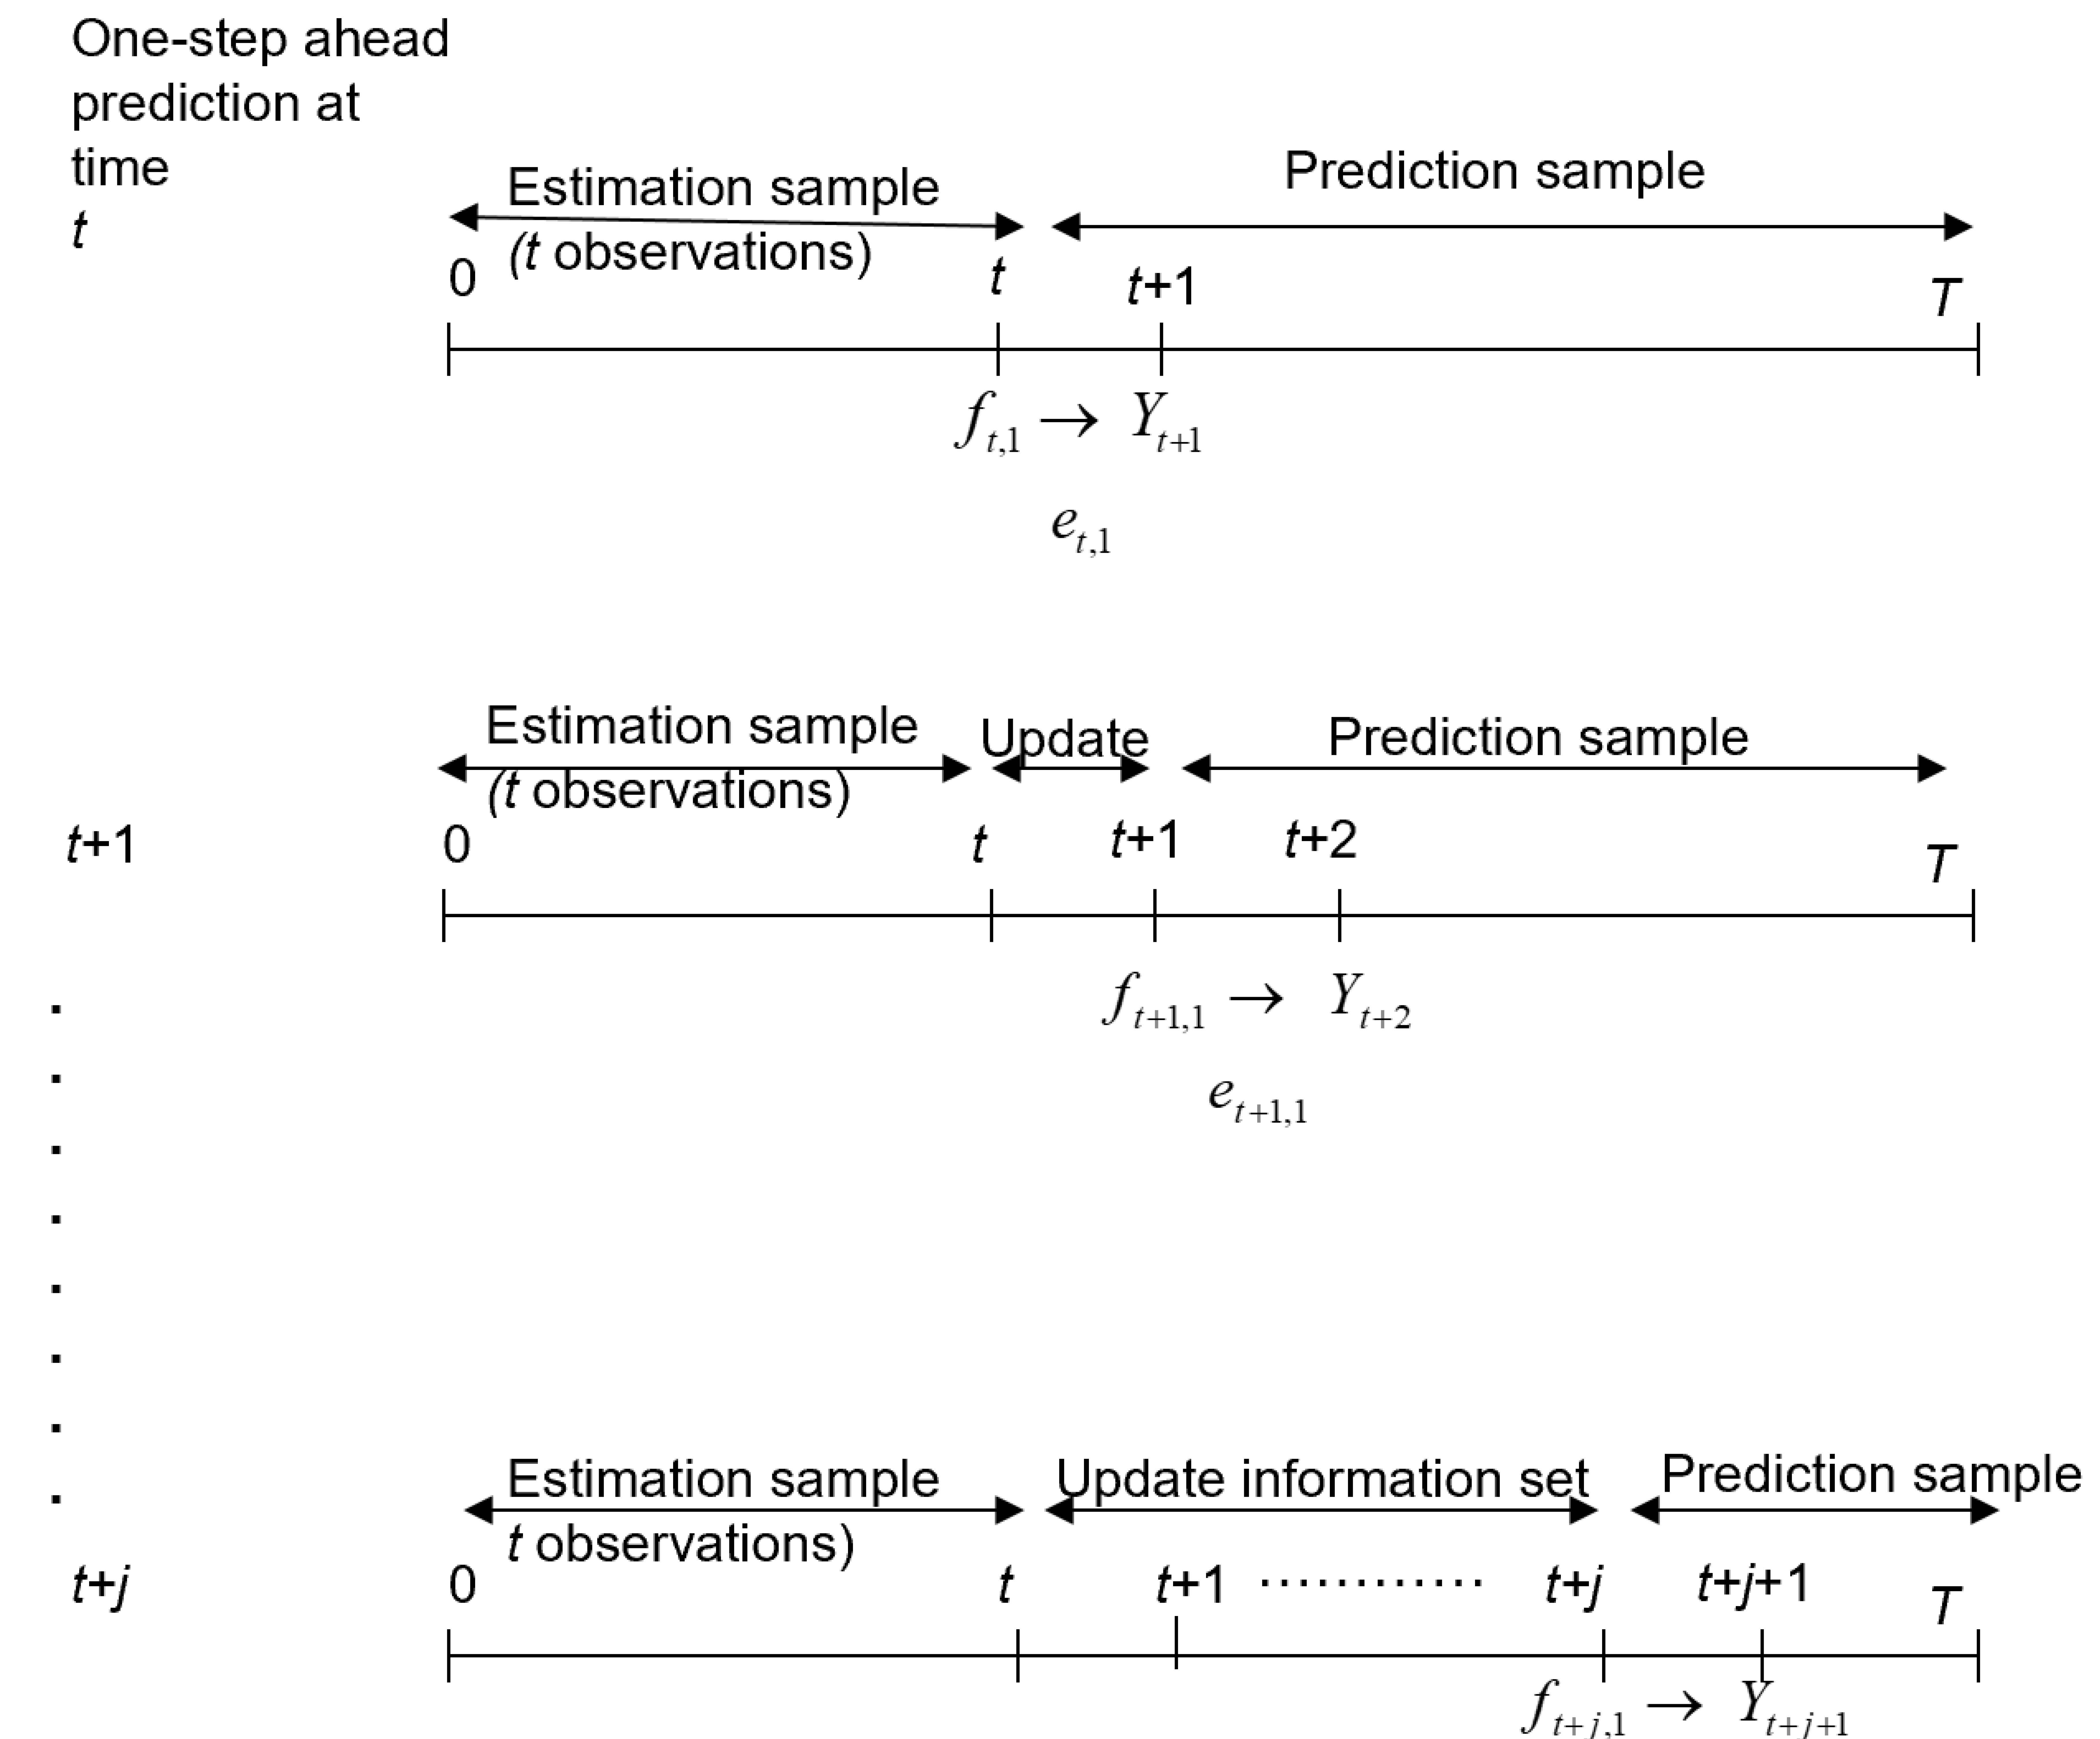
\includegraphics[width=0.5\linewidth]{figures/fixed_forecast}
				\caption{Fixed Forecasting Scheme}
			\end{figure}
	\subsection{Loss Function}
		\begin{definition}
			A loss function $L(e)$ is a real-valued function defined on the space of \emph{forecast errors}, $\mc{E}$, and satisfies the following properties
			\begin{enumerate}[(i)]
				\item $L(e) = 0 \iff \norm{e} = 0$;
				\item $\forall e \in \mc{E}, L(e) \geq 0$\footnote{Since forecasting here can be considered as an optimization process, with $L$ as the objective function. It's fine for $L$ not satisfying the non-negativity condition. However, by convention, we assume $L$ to be non-negative.};
				\item $L$ is \emph{monotonically increasing} in the \emph{norm} of forecast error.
			\end{enumerate}
		\end{definition}
		
		\begin{example}[Symmetric Loss Functions with $\mc{E} = \R$]
			\begin{align}
				L(e) = a e^2,\ a > 0 \\
				L(e) = a\ |e|,\ a > 0
			\end{align}
		\end{example}
		
		\begin{example}[Asymmetric Loss Functions with $\mc{E} = \R$]
			\begin{align}
				L(e) = \exp(ae) - ae - 1,\ a > 0 & \tx{ Lin(ear)-ex(ponential) Function} \\
				L(e) = a\ |e|\ \mathbb{I}(e \geq 0) + b\ |e|\ \mathbb{I}(e < 0) &\tx{ Lin-lin Function}
			\end{align}
		\end{example}
		
	\subsection{Optimal Forecast}
		\begin{definition}
			Based on information set $I_t$, the optimal forecast for future value $y_{t+h}$ is the $f^*_{t,h}$ minimize the \hl{expected loss function}
			\begin{equation}
				\expect{L|I_t} = \int L(y_{t+h} - \red{f_{t,h}}) f(y_{t+h})\ dy_{t+h}
			\end{equation}
		\end{definition}
		
		\begin{assumption}
			Assuming the forecast $f(y_{t+h}|I_t)$ follows
			\begin{equation}
				f(y_{t+h}|I_t) \sim \mc{N}(\expect{Y_{t+h}|I_t}, \var{Y_{t+h}|I_t})
			\end{equation}
		\end{assumption}
		
		\begin{proposition}
			Given \hl{symmetric} quadratic $L$, the optimal forecast $f^*_{t,h}$ is 
			\begin{equation}
				\mu_{t+h|t} \equiv \expect{Y_{t+h}|I_t}
			\end{equation}
			\begin{proof}
				\begin{gather}
					\min_{f_{t, h} \in \R} L \equiv \int (y_{t+h} - f_{t, h})^2 f(y_{t+h}|I_t)\ dy_{t+h} \\
					\pd{L}{f_{t, h}} = -2 \int (y_{t+h} - f_{t, h}) f(y_{t+h}|I_t)\ dy_{t+h} = 0 \\
					\implies \int (y_{t+h} - f_{t, h}) f(y_{t+h}|I_t)\ dy_{t+h} = 0 \\
					\implies \int y_{t+h} f(y_{t+h}|I_t)\ dy_{t+h} = f_{t, h} \int  f(y_{t+h}|I_t)\ dy_{t+h} \\
					\implies \red{f_{t, h} := \mu_{t+h|t} := \expect{y_{t+h}|I_t}}
				\end{gather}
			\end{proof}
		\end{proposition}
		
	\section{Moving Average Process}
		\subsection{Wold Decomposition Theorem}
			\begin{theorem}[Wold Decomposition Theorem]
				Every \ul{covariance stationary} stochastic process $\{Y_t\}$ with mean zero and finite positive variance can be \ul{uniquely} represented as
				\begin{equation}
					Y_t = \underbrace{V_t}_{\tx{AR}} + \underbrace{\sum_{j=0}^\infty \psi_j L^j \varepsilon_t}_{\tx{MA}} = V_t + \Psi(L)\varepsilon_t
				\end{equation}
				where 
				\begin{enumerate}[(i)]
					\item $\{V_t\}$ is a \emph{deterministic component} (e.g. trend or cycle);
					\item $\varepsilon_t \sim \tx{WN}(0, \sigma^2)$ is the \emph{stochastic component};
					\item $\psi_0 = 1$\footnote{We can always normalize $\psi_0$ to 1.} and $\sum_{j=0}^\infty \psi_j^2 < \infty$;
					\item $\expect{\varepsilon_t, V_s} = 0\ \forall t, s \in \mc{T}$.
				\end{enumerate}
			\end{theorem}
			\begin{definition}
				The stochastic component $\{\varepsilon_t\}$ in the decomposition is called \textbf{random shocks} or \textbf{innovations}.
			\end{definition}
			
			\begin{lemma}
				Given $\sum_{j=0}^\infty \psi_j^2 < \infty$, then for all $\varepsilon > 0$ there exists a natural number $J$ such that
				\begin{equation}
					\sum_{j=J}^\infty \psi_j^2 < \varepsilon
				\end{equation}
			\end{lemma}
			
			\begin{corollary}
				By above lemma, assuming $V_t = 0$, we can approximate the decomposition by a linear combination of finite innovations.
				\begin{equation}
					Y_t \approx \hat{Y}_t = \sum_{j=0}^n \psi_j L^j \varepsilon_t
				\end{equation}
				and the approximation is \emph{accurate in Euclidean norm}, that's,
				\begin{equation}
					\expect{Y_t -\sum_{j=0}^n \psi_j L^j \varepsilon_t}^2 \rightarrow 0 \tx{ as } n \to \infty
				\end{equation}
			\end{corollary}
			
			\begin{corollary}
				The Wold decomposition guarantees that there always exists a \ul{linear model} that can represent the dynamics of a \ul{covariance stationary} process.
			\end{corollary}
		\subsection{Moving Average Process}
			\begin{definition}
				The \textbf{Moving Average} of order $q$ with deterministic trend, MA($q$), process is defined by the following stochastic difference equation
				\begin{equation}
					Y_t = \mu + \Theta(L) \varepsilon_t = \mu + \theta_0 \varepsilon_t + \theta_1 \varepsilon_{t-1} + \dots + \theta_q \varepsilon_{t-q} \tx{ where } \theta_0 = 1, \theta_q \neq 0
				\end{equation}
				where $\{\varepsilon_t\}$ is the series of innovations.
			\end{definition}
			
			\begin{lemma}
				The infinite lag polynomial in $\Psi(L)$ can be approximated by
				\begin{equation}
					\Psi(L) \approx \frac{\Theta_q(L)}{\Phi_p(L)}
				\end{equation}
				\begin{proof}[Proof Idea.]
					Taylor's Series.
				\end{proof}
			\end{lemma}
			
			\begin{remark}
				MA process is always \emph{causal} by definition.
			\end{remark}
			
			\begin{definition}
				MA(1) process takes the form of 
				\begin{equation}
					Y_t = \mu + \varepsilon_t + \theta \varepsilon_{t-1}
				\end{equation}
			\end{definition}
			
			\paragraph{Unconditional Moments of MA(1)}where $\mu :=$ unconditional mean.
				\begin{align}
					\expect{Y_t} = \expect{\mu + \varepsilon_t + \theta \varepsilon_{t-1}} &= \mu 
				\end{align}
				\begin{align}
					\var{Y_t} &= \expect{(\varepsilon_t + \theta \varepsilon_{t-1})^2} \\
					&= \var{\varepsilon_t} + \theta^2 \var{\varepsilon_{t-1}} \\
					&= (1 + \theta^2) \sigma_\varepsilon^2
				\end{align}
			\paragraph{Auto-covariance}
				\begin{align}
					\gamma_0 &= \var{Y_t} = (1 + \theta^2) \sigma_\varepsilon^2\\
					\gamma_1 &= \expect{(Y_t - \mu) (Y_{t-1} - \mu)} \\
					&= \expect{(\varepsilon_t + \theta \varepsilon_{t-1})(\varepsilon_{t-1} + \theta \varepsilon_{t-2})} \\
					&= \theta \sigma_\varepsilon^2 \\
					\gamma_k &= 0\ \forall k > 1
				\end{align}
			\paragraph{Auto-correlation}
				\begin{align}
					\rho_1 &= \frac{\gamma_1}{\gamma_0}
					= \frac{\theta}{1 + \theta^2} \\
					\rho_k &= 0\ \forall k > 1
				\end{align}
				
			\begin{definition}
				A MA(1) process is \textbf{invertible} if $|\theta| < 1$, so that it can be written as an AR($\infty$) process.
			\end{definition}
			\begin{proof}[Inverting]
				Let 
				\begin{equation}
					Y_t = \mu + \varepsilon_t + \theta \varepsilon_{t+1}
				\end{equation}
				where $|\theta| < 1$.
				Then, 
				\begin{gather}
					Y_t = \mu + \varepsilon_t + \theta \varepsilon_{t+1} \\
					\implies Y_t - \mu = (1 + \theta L) \varepsilon_t \\ 
					\implies \frac{Y_t - \mu}{1 - (- \theta L)} = \varepsilon_t \\
					\implies \varepsilon_t = (Y_t - \mu) \sum_{j=0}^\infty (-\theta L)^j
				\end{gather}
			\end{proof}
			
			\paragraph{Equivalence} note that for MA(1) process,
				\begin{equation}
					r_1 = \rho_1 = \frac{\theta}{1 + \theta^2}
				\end{equation}
				and for any $\theta$, $\frac{1}{\theta}$ will generate the same auto-correlation. \hl{We always choose the invertible MA representation with $|\theta| < 1$}.
			\begin{proposition}
				For any process, $\rho_1 = r_1$.
			\end{proposition}
			\begin{remark}
				If the MA process is invertible, we can always find an autoregressive representation in which the present is a function of the past innovations.
			\end{remark}
		\subsection{Forecasting with MA(1)}
			\subsubsection{Forecasting with Horizon $h=1$}
				\paragraph{Point estimate}
					\begin{gather}
						f_{t,1} = \expect{Y_{t+1}|I_t} \\
						= \expect{\mu + \theta \varepsilon_{t} + \varepsilon_{t+1}|I_t} \\
						= \mu + \theta \varepsilon_t
					\end{gather}
				\paragraph{Forecasting error}
					\begin{gather}
						e_{t,1} = Y_{t+1} - f_{t,1} = \varepsilon_{t+1}
					\end{gather}
				\paragraph{Forecasting uncertainty}
					\begin{gather}
						\red{\sigma_{t+1|t}^2} = \var{Y_{t+1}|I_t} \\
						= \expect{\varepsilon_{t+1}^2|I_t} \\
						= \sigma^2_\varepsilon
					\end{gather}
				\textbf{Density forecast} assuming \emph{normality} of $\varepsilon$. Confidence interval can be computed using the the density forecast.
					\begin{gather}
						\mc{F} \equiv \mc{N}(\mu_{t+1|t}, \sigma_{t+1|t}^2) \\
						\mu_{t+1|t} = \mu + \theta \varepsilon_t \\
						\sigma_{t+1|t}^2 =  \sigma^2_\varepsilon
					\end{gather}
			\subsubsection{Forecasting with Horizon $h=2$}
				\paragraph{Point estimate}
					\begin{gather}
						f_{t,2} = \expect{Y_{t+2} | I_t} \\
						= \expect{\mu + \theta \varepsilon_{t+1} + \varepsilon_{t+2} | I_t}
						= \mu
					\end{gather}
				\textbf{Forecasting error}
					\begin{gather}
						Y_{t+2} - f_{t,2} = \theta \varepsilon_{t+1} + \varepsilon_{t+2}
					\end{gather}
				\textbf{Forecasting Uncertainty}
					\begin{gather}
						\sigma_{t+2|t}^2 \equiv \var{Y_{t+2} | I_t} \\
						= (1 + \theta^2) \sigma_{\varepsilon}^2 
					\end{gather}
				\textbf{Density forecast}
					\begin{gather}
						\mc{F} = \mc{N}(\mu, (1 + \theta^2)\sigma_{\varepsilon}^2)
					\end{gather}
				\begin{remark}
					Since for any $h > 1$, MA(1) only generates the unconditional mean $\mu$ as the point estimate, we say MA(1) process is \textbf{short memory}.
				\end{remark}
		\subsection{Properties of MA(2) Process}
			\paragraph{Model}
				\begin{equation}
					Y_t = \mu + \varepsilon_t + \theta_1 \varepsilon_{t-1} + \theta_2 \varepsilon_{t-2}
				\end{equation}
			\paragraph{Unconditional Moments}
				\begin{gather}
					\expect{Y_t} = \mu \\
					\var{Y_t} = (1 + \theta_1^2 + \theta_2^2) \sigma_\varepsilon^2
				\end{gather}
			\paragraph{Auto-covariance}
				\begin{gather}
					\gamma_0 = \var{Y_t} = (1 + \theta_1^2 + \theta_2^2) \sigma_\varepsilon^2 \\
					\gamma_1 = (\theta_1 + \theta_1 \theta_2) \sigma_\varepsilon^2 \\
					\gamma_2 = \theta_2 \sigma_\varepsilon^2
				\end{gather}
			\paragraph{Auto-correlation}
				\begin{gather}
					\rho_1 \equiv \frac{\gamma_1}{\gamma_0} = \frac{\theta_1 + \theta_1 \theta_2}{1 + \theta_1^2 + \theta_2^2} \\
					\rho_2 \equiv \frac{\gamma_2}{\gamma_0} = \frac{\theta_2}{1 + \theta_1^2 + \theta_2^2}
				\end{gather}
			\paragraph{Optimal Forecasting}
				\begin{gather}
					f_{t, 1} = \mu + \theta_1 \varepsilon_t + \theta_2 \varepsilon_{t-1} \\
					f_{t, 2} = \mu + \theta_2 \varepsilon_t \\
					f_{t, h} = \mu\ \forall h > 2
				\end{gather}
			
		\subsection{MA Forecasting Procedure}
			\begin{remark}
				Assuming the MA process used is invertible, we use its inverting representation to recover $\hat{\varepsilon}_t$.
			\end{remark}
	
	\section{Auto-Regression Process and Seasonality}
		\subsection{AR Process}
			\begin{definition}
				An \textbf{auto-regressive} model of order $p$ is taken in the form of 
				\begin{equation}
					Y_t = c + \sum_{j=1}^p \phi_j L^j Y_t + \varepsilon_t
				\end{equation}
				or equivalently
				\begin{equation}
					\Phi_p(L) Y_t = c + \varepsilon_t
				\end{equation}
			\end{definition}
			
			\begin{definition}
				An \textbf{auto-regressive} process of order 1 takes the form of \emph{stochastic difference equation}:
				\begin{equation}
					Y_t = c + \phi Y_{t-1} + \varepsilon_t
				\end{equation}
				where $\phi$ is called the \textbf{persistence parameter}.
			\end{definition}
		
		\begin{proposition}
			AR(1) process is stationary if and only if $|\phi| < 1$ (\emph{all roots outside the unit circle}).
		\end{proposition}
		
		\paragraph{ACF and PACF}
			\begin{gather}
				\rho_1 = r_1 = \phi \\
				r_k = 0\ \forall k > 1
			\end{gather}
			
		\subsubsection{Forecasting with AR(1) and $h=1$}
			\begin{assumption}
				While examining the optimal forecast in this section, we are assuming the loss function is \emph{symmetric}.
			\end{assumption}
			
			\paragraph{Point estimate}
				\begin{gather}
					f_{t,1} = \expect{Y_{t+1}|I_t} \\
					= c + \phi Y_t
				\end{gather}
			\paragraph{Forecast variance(uncertainty)}
				\begin{gather}
					\var{Y_{t+1}|I_t} = \var{c + \phi Y_t + \varepsilon_{t+1}|I_t}
					= \sigma_\varepsilon^2
				\end{gather}
			\textbf{Density forecast}
				\begin{gather}
					\mc{F} = \mc{N}(c + \phi Y_t, \sigma_\varepsilon^2)
				\end{gather}
				
		\subsubsection{Forecasting with AR(1) and $h=s>1$}
			\paragraph{Point estimate}
				\begin{gather}
					f_{t,s} = \expect{Y_{t+s}|I_t} \\
					= c + \expect{\phi Y_{t+s-1}|I_t} \\
					= (1 + \phi + \dots + \phi^{s-1}) c + \phi^s Y_t
				\end{gather}
			\textbf{Forecasting uncertainty}
				\begin{gather}
					\var{Y_{t+s}|I_t} = \var{\varepsilon_{t+s} + \phi \varepsilon_{t+s-1} + \dots + \phi^{s-1} \varepsilon_{t+1} | I_t} \\
					= \sum_{j=0}^{s-1} \phi^{\red{2j}} \sigma_\varepsilon^2
				\end{gather}
			\begin{remark}
				\emph{ACF and PACF are estimated functions subject to sampling error, so the estimated ACF and PACF from sample might be different from their theoretical values.}
			\end{remark}
		\subsubsection{Forecasting with AR(1) and $h \to \infty$}
			\begin{assumption}
				For this subsection, assuming the AR(1) process is \hl{stationary}, that's, $|\phi| < 1$.
			\end{assumption}
			\textbf{Point Estimate}
				\begin{gather}
					\lim_{h \to \infty} f_{t, h} = \frac{c}{1 - \phi}
				\end{gather}
			\textbf{Forecasting Uncertainty}
				\begin{gather}
					\lim_{h \to \infty} \var{Y_{t+h}|I_t} = \frac{\sigma_\varepsilon^2}{1 - \phi^2}
				\end{gather}
			\begin{remark}
				The convergences demonstrated above suggest auto-regressive process is still a \textbf{short memory} process.
			\end{remark}
			
		\subsubsection{Forecasting with AR(2) process}
			\begin{definition}
				AR(2) process
				\begin{equation}
					Y_t = c + \phi_1 Y_{t-1} + \phi_2 Y_{t-2} + \varepsilon_t
				\end{equation}
			\end{definition}
			\paragraph{Unconditional Moments}
				\begin{gather}
					\expect{Y_t} = c + \phi_1 \expect{Y_{t-1}} + \phi_2 \expect{Y_{t-2}} \\
					\implies \red{\mu_Y = \frac{c}{1 - \phi_1 - \phi_2}}
%					\var{Y_t} = \sigma_\varepsilon^2
				\end{gather}
			\paragraph{Auto-covariance and Auto-correlation}
				\begin{gather}
					\rho_1 = r_1 \\
					r_2 = \phi_2 + \red{\text{ sampling error}}
				\end{gather}
			\paragraph{Optimal Forecasts $h=1$}
				\begin{gather}
					f_{t,1} = \expect{Y_{t+1}|I_t} \\
					= \expect{c + \phi_1 Y_t + \phi_2 Y_{t-1} + \varepsilon_{t+1}|I_t} \\
					= c + \phi_1 Y_t + \phi_2 Y_{t-1}
				\end{gather}
				\begin{gather}
					e_{t,1} = \varepsilon_{t+1}
				\end{gather}
				\begin{gather}
					\sigma_{t+1|t}^2 = \var{Y_{t+1}|I_t} = \sigma_\varepsilon^2
				\end{gather}
			\paragraph{Optimal Forecasts $h=2$}
				\begin{gather}
					f_{t,2} = \expect{Y_{t+2}|I_t} \\
					= \expect{c + \phi_1 Y_{t+1} + \phi_2 Y_t + \varepsilon_{t+2}|I_t} \\
					= c + \phi_1 \red{f_{t,1}} + \phi_2 Y_t 
				\end{gather}
				\begin{gather}
					e_{t,2} = Y_{t+2} - f_{t,2} \\
					= \phi_1 (Y_{t+1} - f_{t,1}) + \varepsilon_{t+2} \\
					= \phi_1 e_{t,1} + \varepsilon_{t+2}
				\end{gather}
				\begin{gather}
					\sigma_{t+2|t}^2 = \var{Y_{t+2}|I+t} \\
					= \phi_1^2 \sigma_{t+1|t}^2 + \sigma_\varepsilon^2 \\
					= (1 + \phi_1^2) \sigma_\varepsilon^2
				\end{gather}
			\textbf{Optimal Forecasts $h=s>2$}
				\begin{align}
					f_{t, s} &= \expect{Y_{t+s}|I_t} \\
					&= c + \phi_1 f_{t, s-1} + \phi_2 f_{t, s-2}
				\end{align}
				
				\begin{align}
					e_{t, s} &= \phi_1(Y_{t+s-1} - f_{t, s-1}) + \phi_2(Y_{t+s-2} - f_{t, s-2}) + \varepsilon_{t+s} \\
					&= \phi_1 e_{t, s-1} + \phi_2 e_{t, s-2} + \varepsilon_{t+s}
				\end{align}
				
				\begin{align}
					\sigma_{t+s|t}^2 &= \var{Y_{t+s}|I_t} \\
					&= \var{e_{t,s}|I_t} \\
					&= \phi_1 \sigma_{t+s-1|t}^2 + \phi_2 \sigma_{t+s-2|t}^2 + \sigma_\varepsilon^2
				\end{align}
			\begin{remark}
				AR(2) is still classified as \emph{short memory processes} as 
				\begin{align}
					\lim_{s \to \infty} f_{t, s} &= \mu \\
					\lim_{s \to \infty} \sigma_{t+2|t}^2 &= \sigma_Y^2
				\end{align}
			\end{remark}
			
		\subsubsection{AP($p$) process}
			\begin{definition}
				Let $\Phi(L)Y_t = c + \varepsilon_t$ be an AR($p$) process with trend $c$, then $\Phi(\cdot)$ is called the \textbf{characteristic polynomial} of this stochastic process.
			\end{definition}
			
			\begin{theorem}
				An autoregressive process is stationary \ul{if and only if} all roots of its characteristic polynomial are \hl{outside} the unit circle on $\C$.
			\end{theorem}
			
			\paragraph{Forecasting with AR($p$) Process} we apply a \hl{recursive} scheme, or \hl{\textbf{chain rule of forecasting}}, in which the we use the \emph{forecasted} values to make prediction on even further values.
			\begin{example}[AP($p$) chain rule of forecasting]
				\begin{align}
					\red{f_{t,1}} &= c + \sum_{j=1}^p \phi_j L^j Y_{t+1} \\
					\orange{f_{t,2}} &= c + \phi_1 \red{f_{t,1}} + \sum_{j=2}^p \phi_j L^j Y_{t+2} \\
					\blue{f_{t,3}} &= c + \phi_1 \orange{f_{t,2}} + \phi_2 \red{f_{t,1}} + \sum_{j=3}^p \phi_j L^j Y_{t+3}\\
					f_{t, s} &= c + \sum_{j=1}^p \phi_j f_{t, s-j}\ \forall s > p
				\end{align}
			\end{example}
		
		\subsection{Procedures of Forecasting with Autoregressive Models}
			\begin{enumerate}[(i)]
				\item \textbf{Estimate} $\hat{\Phi}$ and $\hat{\sigma}_\varepsilon^2$ and $\hat{\mu}$ (unconditional mean). 
				\item Calculate $\hat{c}$(intercept) from $\hat{\Phi}$ and $\hat{\mu}$.
				\item Construct forecast $f_{t, h}$ with \textbf{chain rule of forecasting}.
				\item \textbf{Density forecast}, under normality assumption of $\varepsilon$ is
				\begin{equation}
					\mc{N}(f_{t,h}, \hat{\sigma}^2_{t+h|t})
				\end{equation}
				\item 95\% confidence interval of forecasting is
				\begin{equation}
					(f_{t,h} \pm 1.96 \times \hat{\sigma}_{t+h|t})
				\end{equation}
			\end{enumerate}
		
		\subsection{Seasonality}
			\subsubsection{Deterministic Seasonality}
				\begin{definition}
					The seasonality is \textbf{deterministic} if the seasonal component regressors are always exactly predictable.
				\end{definition}
				
				\begin{remark}
					To handle deterministic seasonality, just add those indicator terms into the regression.
				\end{remark}
				
			\subsubsection{Stochastic Seasonality}
				\begin{definition}
					The seasonality is \textbf{stochastic} if the seasonal component is driven by random variables.
				\end{definition}
				
				\begin{definition}
					A seasonal AP($p$) model, S-AR($p$), is defined by
					\begin{gather}
						Y_t = c + \phi_s Y_{t-s} + \phi_{2s} + Y_{t-2s} + \dots + \phi_{ps} Y_{t - ps} + \varepsilon_t \\
						\Phi_{p}(L^s) Y_t = c + \varepsilon_t
					\end{gather}
					where $s$ refers to the \textbf{data frequency}. Such model seeks to explain the \textbf{dynamics across seasons}.
				\end{definition}
				
				\begin{definition}
					Characteristics of realizations from S-AR($p$) process:
					\begin{enumerate}[(i)]
						\item ACF decays slowly with spikes at \ul{multiples of $s$}.
						\item PACF \hl{only} spikes at \ul{multiples of $s$}.
					\end{enumerate}
				\end{definition}
				
				\begin{definition}
					A seasonal MA($q$) model, S-MA($q$), is given by
					\begin{equation}
						Y_t = \mu + \Theta_q(L^s) \varepsilon_t
					\end{equation}
				\end{definition}
				
				\begin{remark}
					Characteristics of realizations from S-MA($q$) process:
					\begin{enumerate}[(i)]
						\item ACF \hl{only} spikes at \ul{multiples of $s$}.
						\item PACF decays slowly with spikes at \ul{multiples of $s$}.
					\end{enumerate}
				\end{remark}
				
				\begin{proposition}[Combing ARMA and S-ARMA]
					Given ARMA 
					\begin{equation}
						\Phi_p(L) Y_t = c + \Theta_q(L) \varepsilon_t
					\end{equation}
					and S-ARMA
					\begin{equation}
						\Phi_p'(L^{s_1}) Y_t = c + \Theta_q'(L^{s_2}) \varepsilon_t
					\end{equation}
					The combined model is given by \hl{multiplying the lag polynomials}
					\begin{equation}
						\Phi_p(L) \Phi_p'(L^{s_1}) Y_t = c +  \Theta_q(L) \Theta_q'(L^{s_2}) \varepsilon_t
					\end{equation}
				\end{proposition}
	\section{Model Assessment and Asymmetric Loss}
		\subsection{Model Assessment}
			\begin{definition}
				\textbf{Akaike information criterion}(AIC) of a model with $k$ parameters is defined as
				\begin{equation}
					\red{AIC := -2 \ln(\mc{L}) + 2k}
				\end{equation}
			\end{definition}
			
			\begin{definition}
				\textbf{Bayes information criterion}(BIC)/\textbf{Schwarz information criterion}(SIC) of a model with $k$ parameters and fitted on the sample with size $N$ is defined as
				\begin{equation}
					\red{BIC := -2 \ln(\mc{L}) + 2 \ln(N) k}
				\end{equation}
			\end{definition}
			
			\begin{definition}
				Given time series data sample with size $T$, and use the \emph{recursive scheme} starting from $t < T$, with forecasting horizon $h$, given sequence of \emph{ground truth}
				\begin{equation}
					\mathscr{Y} = (y_j)_{j=t+h}^T
				\end{equation}
				we can construct a sequence of forecast
				\begin{equation}
					\mathscr{F} = (f_{t, h}, f_{t+1, h}, f_{t+2, h}, \dots, f_{T-h, h})
				\end{equation}
				and a sequence of forecasting errors
				\begin{equation}
					\mathscr{E} = (e_{j, t})_{j=t+h}^T
				\end{equation}
				then,
				\begin{gather}
					\tx{MSE} \equiv \frac{1}{|\mathscr{F}|} \sum_{e \in \mathscr{E}} e^2 \\
					\tx{MAE} \equiv \frac{1}{|\mathscr{F}|} \sum_{e \in \mathscr{E}} \norm{e} \\
					\tx{MAPE} \equiv \frac{1}{|\mathscr{F}|} \sum_{(y,e) \in (\mathscr{Y}, \mathscr{E})} \norm{\frac{e}{y}}
				\end{gather}
			\end{definition}
		\subsection{Asymmetric Loss}
			\begin{definition}[Log-Normal Distribution]
				Let $X$ be a Gaussian random variable with mean $\mu$ and variance $\sigma^2$. Define $Y \equiv \exp(X)$, then $Y$ follows \textbf{log-normal distribution}, with 
				\begin{equation}
					\expect{Y} = \exp(\mu + \frac{\sigma^2}{2})
				\end{equation}
			\end{definition}
			
			\begin{example}
				Consider the Lin-ex loss function
				\begin{equation}
					L(e) = \exp(ae) - ae - 1
				\end{equation}
				then the expected loss for $h$ step forecasting made at $t$ is 
				\begin{gather}
					\expect{L(e_{t,h})|I_t} \\
					= \expect{\exp(a(y_{t+h} - f_{t,h})) - a(y_{t+h} - f_{t,h}) - 1|I_t} \\
					= \expect{\exp(a y_{t+h}) \exp(-a f_{t,h})|I_t} - \expect{a y_{t+h}|I_t} + a f_{t,h} - 1 \\ 
					= \exp(-a f_{t,h}) \expect{\exp(a y_{t+h})|I_t} - a \expect{y_{t+h}|I_t} + a f_{t,h} - 1 \\
				\end{gather}
				To find the optimal forecasting, take the FOC
				\begin{gather}
					\pd{\expect{L(e_{t,h})|I_t}}{f_{t,h}} = 0\\
					\implies -a \exp(-a f_{t,h}) \expect{\exp(a y_{t+h})|I_t} + a = 0 \\
					\implies \exp(-a f_{t, h}) \expect{\exp(a y_{t+h})|I_t} = 1 \\
					\implies - a f_{t, h} + \log(\expect{\exp(a y_{t+h})|I_t}) = 0 \\
					\implies f_{t, h} = \frac{1}{a} \log(\expect{\exp(a y_{t+h})|I_t})
				\end{gather}
				Assuming $y_{t+h} \sim \mc{N}(\mu_{t+h|t}, \sigma_{t+h|t}^2)$, 
				\begin{gather}
					\implies f_{t, h} = \frac{1}{a} \log(\exp(
						a \expect{y_{t+h}|I_t} + \frac{a^2 \sigma_{t+h|t}^2}{2}
					)) \\
					\implies f_{t, h} = \expect{y_{t+h}|I_t} + \red{\frac{a \sigma^2_{t+h|t}}{2}}
				\end{gather} 
				So if $a < 0$, the penalty on making negative error is higher than positive error, and the optimal forecast would be \emph{pushed down} to less than the conditional mean.
				\begin{figure}[H]
					\centering
					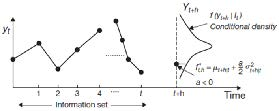
\includegraphics{figures/asym_loss_forecast}
					\caption{Illustration of the Optimal Forecast with Lin-Ex loss and $a < 0$}
				\end{figure}
				\paragraph{Forecasting} Assuming AR(1) process. \\
				\textbf{Error with $h=1$}
					\begin{gather}
						e_{t+1, t} = c + \phi Y_t + \varepsilon_{t+1} - f_{t,1} \\
						= \varepsilon_{t+1} -\frac{a \sigma_{t+1|t}^2}{2} \\
						\expect{e_{t+1, t}} = - \frac{a \sigma_{t+1|t}^2}{2} \\
						\var{e_{t+1,t}|I_t} = \sigma_\varepsilon^2
					\end{gather}
				\textbf{Error with $h=2$}
					\begin{gather}
						e_{t+2, t} = Y_{t+2} - f_{t, 2} \\
						= c + \phi(Y_{t+1}) + \varepsilon_{t+2} - f_{t,2} \\
						= c + \phi c + \phi \varepsilon_{t+1} + \phi Y_t + \varepsilon_{t+2} - f_{t,2} \\
						= c + \phi c + \phi \varepsilon_{t+1} + \phi Y_t + \varepsilon_{t+2} - \expect{Y_{t+2}|I_t} - \frac{a \sigma_{t+2|t}^2}{2} \\
						= \phi \varepsilon_{t+1} + \varepsilon_{t+2} -  \frac{a \sigma_{t+2|t}^2}{2}
					\end{gather}
					Note that for every $h > 0$, the term $\sigma_{t+h|t}$ is constant conditioned on $I_t$.
					\begin{gather}
						\expect{e_{t+2,t}|I_t} = - \frac{a \sigma_{t+2|t}^2}{2} \\
						\var{e_{t+2,t}|I_t} = (1 + \phi^2) \sigma_\varepsilon^2
					\end{gather}
			\end{example}
	
	\section{Trends}
	
	
	\section{Vector Auto-regression Model}
	
	\section{Vector Error Correction Model}
			
	\section{Volatility I}
	
	\section{Volatility II}
	
	\section{Volatility III: Applications}
		\subsection{Risk Management}
			\begin{definition}
				The \textbf{$\alpha$-Value at Risk (VaR)}, $r_t^{VaR(\alpha)}$, is the $\alpha$-quantile of $r_t$.
			\end{definition}
			
			\begin{remark}[Interpretation]
				$r_t^{VaR(\alpha)}$ is the value in the domain of $r_t$ such that \emph{the possibility of obtaining an equal or smaller value than $r_t$ is $\alpha \%$}.
				\begin{equation}
					\prob{r_t \leq r_t^{VaR(\alpha)}} = \alpha
				\end{equation}
			\end{remark}
	
			\paragraph{Model Setup}
				\begin{gather}
					r_t = \mu_{t|t-1} + \sigma_{t|t-1}z_t \\
					z_t \sim \mc{N}(0, 1) \\
					\mu_{t|t-1} \sim \tx{ARMA} \\
					\sigma_{t|t-1} \sim \tx{GARCH} \\
					\implies r_t \sim \mc{N}(\mu_{t|t-1}, \sigma_{t|t-1}^2) \\
					\implies \red{r_t^{VaR(\alpha)} = \mu_{t|t-1} + \Phi^{-1}(\alpha) \sigma_{t|t-1}}
				\end{gather}
				
			\begin{figure}[h]
				\centering
				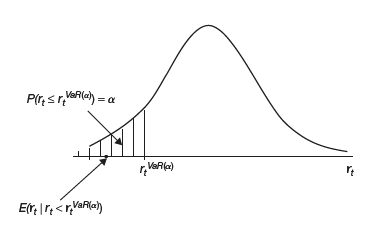
\includegraphics[width=0.7\linewidth]{figures/lec12.png}
				\caption{VaR and Expected Shortfall}
			\end{figure}
			
			\begin{definition}
				The \textbf{expected shortfall} measures the average value of such loss,
				\begin{equation}
					ES(\alpha) := \expect{r_t|r_t < r_t^{VaR(\alpha)}}
				\end{equation}
			\end{definition}
			
			\begin{lemma}[Expected of Truncated Normal Distribution]
				\begin{gather}
					X \sim \mc{N}(\mu, \sigma^2) \\
					\implies \expect{X|a < X < b} = \mu + \sigma \frac{\phi(\frac{a - \mu}{\sigma}) - \phi(\frac{b - \mu}{\sigma})}{\Phi(\frac{b - \mu}{\sigma}) - \Phi(\frac{a - \mu}{\sigma})} \\
					= \red{\mu + \sigma \frac{\phi(\alpha) - \phi(\beta)}{\Phi(\beta) - \Phi(\alpha)}}
				\end{gather}
			\end{lemma}
			
			\begin{proposition}
				Computing the \emph{expected shortfall} with \ul{normality assumption}.
				\begin{gather}
					r_t \sim \mc{N}(\mu_{t|t-1}, \sigma_{t|t-1}^2) \\
					\implies \red{\expect{r_t|r_t < r_t^{VaR(\red{\alpha})}}}  = \mu_{t|t-1} + \sigma_{t|t-1} 
					\frac{-\phi \left( 
						\frac{r_t^{VaR(\alpha)} - \mu_{t|t-1}}{\sigma_{t|t-1}}
					\right)}
					{\Phi \left(
						\frac{r_t^{VaR(\alpha)} - \mu_{t|t-1}}{\sigma_{t|t-1}} 
					\right)} \tx{ (by equation (7.7))}\\
					= \red{\mu_{t|t-1} - \sigma_{t|t-1} \frac{\phi(\Phi^{-1}(\alpha))}{\alpha}}
				\end{gather}
				with R-code \texttt{coef <- dnorm(pnorm(alpha))/alpha}.
			\end{proposition}
		
		\subsection{Portfolio Allocation}
			\paragraph{The Problem}Suppose there are two assets (can be easily extend to the general case, let $N$ denote the set of assets). Returns associated with those assets have mean $\mu_i$ and variance $\sigma_i^2$ for each $i \in N$. For given level of $\overline{\mu}_p$, one has to choose $(w_i)_{i \in N}$ such that the risk, $\sigma^2_p$, is minimized.
			
			\begin{assumption}
				\begin{gather}
					Cov(r_i, r_j) = 0\ \forall i \neq j \in N
				\end{gather}
			\end{assumption}
			
			\paragraph{Solution}
			\begin{gather}
				\min_{(w_i)_{i \in N}} \sigma_p^2 \equiv \sum_{i \in N} w_i^2 \sigma_i^2 \\
				s.t.\ \overline{\mu}_p = \sum_{i \in N} w_i \mu_i \\
				\implies w_i^* = \frac{
					\mu_i/\sigma_i^2
				}{
					\sum_{j \in N} \mu_j/\sigma_j^2
				}\overline{\mu}_p
			\end{gather}
			
			\begin{remark}
				The means and variances of assets can be estimated \emph{conditionally on $t$} using the hybrid $ARMA-GARCH$ model.
			\end{remark}
		
		\subsection{Asset Pricing: Classical Capital Asset Pricing Model}
			\begin{definition}
				A \textbf{market portfolio} is a theoretical bundle of investments that includes every type of asset available in the world financial market, with each asset weighted in proportion to its total presence in the market.
			\end{definition}
			
			\begin{proposition}
				\begin{gather}
					\expect{r_i} = r_f + \beta_i \expect{r_m - r_f} \\
					\beta_i := \frac{Cov(r_i, r_m)}{Var(r_m)} \equiv \frac{\rho_{im}\sigma_i \sigma_m}{\sigma_m^2}
				\end{gather}
				and if $\beta_i > 1$, the asset $i$ is more \emph{risky} than the market risk. In practice, $\beta_i$ is estimated with $\rho_{im}$ estimated directly from samples and $\sigma^2_{i, t|t-1}, \sigma^2_{mz, t|t-1}$ estimated using $GARCH$.
			\end{proposition}
	
	\section{Nonlinear Models}
		\subsection{Threshold Auto-Regression (TAR)}
			\begin{definition}
				Given data structure containing \textbf{main/target series}
				\begin{gather}
					\{y_t\}
				\end{gather}
				and \textbf{threshold/activation variable series}
				\begin{equation}
					\{x_t\}
				\end{equation}
				To construct a $TAR(p)$ model with $r$ regimes, 
				\begin{enumerate}[(i)]
					\item Partitioning the range of $X_t$ (typically $\R$) into $r$ \emph{disjoint} sets $\{R_i\}_{i=1}^r$.
					\item Construct model using indicator functions
					\begin{equation}
						Y_t = \sum_{i=1}^r \mathds{1}\{x_{\red{t}} \in R_i\} 
						\underbrace{\left(
							\phi_{i0} + \sum_{j=1}^p \phi_{ij} Y_{t-j} + \varepsilon_{it}
						\right)}_{\tx{Regim $i$ AR($p$) Model}}
					\end{equation}
				\end{enumerate}
			\end{definition}
		
			\begin{definition}
				If the threshold/activation variable in a TAR model is any \emph{lagged variation of the main/target series}, then the TAR model is called \textbf{self-exciting}.
			\end{definition}
		
		\subsection{Test Significance of Regimes}
			\begin{remark}
				To \ul{test the significance of multiple regimes}, we use conventional hypothesis testing for significance of coefficients in multiple regression models.
			\end{remark}
			\begin{example}
				To test the significance (whether it is necessary to include it) of two regimes (but with same error term) here 
				\begin{align}
					Y_t &= \mathds{1}\{ Y_{t-1} \geq 0\} 
					\left ( 
						\phi_0 + \phi_1 Y_{t-1}
					\right )
					+ 
					\mathds{1}\{ Y_{t-1} < 0\} 
					\left ( 
						\phi_0' + \phi_1' Y_{t-1}
					\right ) + \varepsilon_t \\
					D_t &:= \mathds{1}\{ Y_{t-1} \geq 0\} \\
					\implies Y_t &= D_t \left (\phi_0 + \phi_1 Y_{t-1}\right ) + (1 - D_t) \left (\phi_0' + \phi_1' Y_{t-1}\right ) + \varepsilon_t \\
					\implies Y_t &= \phi_0' + \phi_1' Y_{t-1} + (\underbrace{\phi_0 - \phi_0'}_{\Delta \phi_0}) D_t + (\underbrace{\phi_1 - \phi_1'}_{\Delta \phi_1}) D_t Y_{t-1} + \varepsilon_t
				\end{align}
				And test the hypothesis (equivalently, \ul{test the \emph{joint significance} of coefficients of $D_t$ and $D_t Y_{t-1}$}
				\begin{align}
					H_0 &:= \Delta \phi_0 = 0 \land \Delta \phi_1 = 0 \tx{ model is linear}\\
					H_1 &:= \neg H_0 \tx{ model is non-linear}
				\end{align}
			\end{example}
			
		\subsection{Smooth Transition Autoregressive Model (STAR)}
			\begin{definition}
				A \textbf{smooth transition autoregressive model}(STAR) is defined by two autoregression regimes and a \emph{bounded and continuous} (activation function) $\mc{G}(s_t, \gamma, c)$. Where 
				\begin{enumerate}[(i)]
					\item $\gamma$ denotes the \textbf{speed parameter};
					\item $c$ denotes \textbf{threshold};
					\item $\mc{G}$ is bounded and continuous in \textbf{threshold variables} $s_t$.
				\end{enumerate}
				\begin{gather}
					Y_t = \underbrace{\left(
						\phi_0 + \sum_{j=1}^p \phi_j L^j Y_t
					\right)}_{\text{base model}} + 
					\underbrace{\left(
						\phi_0' + \sum_{j=1}^p \phi_j' L^j Y_t
						\right)
						\red{\mc{G}(s_t, \gamma, c)}
					}_{\text{activation}}
					+ \varepsilon_t
				\end{gather}
			\end{definition}
			
			\begin{example}[STAR(1) without intercept]
				\begin{gather}
					Y_t = \phi_0 Y_{t-1} + \phi_1 Y_{t-1} \mc{G}(s_t, \gamma, c) + \varepsilon_t
				\end{gather}
			\end{example}
			
			\begin{example}[Logistic STAR]
				\begin{gather}
					\mc{G}(s_t, \gamma, c) = \frac{1}{1 + \exp(-\gamma(s_t - c))}
				\end{gather}
			\end{example}
			
			\begin{example}[Exponential STAR]
				\begin{gather}
					\mc{G}(s_t, \gamma, c) = 1 - \exp(-\gamma (s_t - c)^2)
				\end{gather}
			\end{example}
			
			\begin{remark}
				STAR is effectively a TAR with infinitely many regimes.
			\end{remark}
		
		\subsection{Markov Switching Model}
			\begin{definition}
				MS models the \emph{probability of various regimes to happen}. A Markov switching model consists both
				\begin{enumerate}[(i)]
					\item \textbf{State space} $\Omega := \{\omega_i\}_{i=1}^n$;
					\item \textbf{Outcome} functions depend on state realized at time $t$, $s_t$;
						\begin{equation}
							Y_t \sim \mc{N}(\mu_i, \sigma^2) \tx{ if } s_t = \omega_i
						\end{equation}
					\item A $n \times n$ \textbf{transition matrix} $T$ defined as
					\begin{equation}
						T[i, j] := \prob{s_t = \omega_j|s_{t-1} = \omega_i} 
					\end{equation}
				\end{enumerate}
			\end{definition}
\end{document}
































